% !TeX program = lualatex
% ---------------------------------------------------------------
%  Geometria — Samarang, 28 November 1787
%  Nationaal Archief 1.04.02, inv. 3775, fol. 3599–3607
%  GLOBALISE scans 0032–0040
%
%  Compile with LuaLaTeX (or XeLaTeX): unicode text and Greek are
%  set directly; EB Garamond is loaded through fontspec.
%      lualatex geometria.tex
%
%  Self-contained: enumitem.sty, needspace.sty and footnote.sty are
%  vendored beside this file (TeX Live "basic" ships none of them), and
%  EB Garamond lives in fonts/ as the OFL variable faces, so no system
%  install is needed.
% ---------------------------------------------------------------
% openany: the front matter runs straight through to the first example, with no
% blank versos forced in front of the two opening chapters.
\documentclass[11pt,twoside,openany]{book}

\usepackage{fontspec}
\usepackage{amsmath,amssymb}
\usepackage{cancel}
\usepackage{tikz}
\usepackage[a4paper,inner=28mm,outer=24mm,top=26mm,bottom=26mm]{geometry}
\usepackage{xcolor}
\usepackage{enumitem}
\usepackage{fancyhdr}
\usepackage{needspace}
% Lets \footnote survive being written inside a box: see \wnote below.
\usepackage{footnote}
\usepackage{microtype}
\usepackage[hidelinks]{hyperref}

% Variable faces: the weight axis supplies bold, so only two files are needed.
\setmainfont{EBGaramond-var.ttf}[
  Path              = ./fonts/,
  UprightFeatures   = {RawFeature={axis={wght=400}}},
  ItalicFont        = EBGaramond-Italic-var.ttf,
  ItalicFeatures    = {RawFeature={axis={wght=400}}},
  BoldFont          = EBGaramond-var.ttf,
  BoldFeatures      = {RawFeature={axis={wght=700}}},
  BoldItalicFont    = EBGaramond-Italic-var.ttf,
  BoldItalicFeatures= {RawFeature={axis={wght=700}}}]

% Vulgar fractions. EB Garamond builds these from a plain solidus via the
% OpenType `frac` feature (slash -> fraction, digits -> numerator/denominator
% forms). A literal U+2044 does not trigger it and collides with lining digits,
% so fractions must be written \vfrac{1}{9}, never with a literal U+2044.
\newcommand{\vfrac}[2]{{\addfontfeature{Fractions=On}#1/#2}}

% The scribe's circle and proportion signs. EB Garamond has neither U+2299 nor
% U+2237, and a missing character is dropped silently, so both must be built.
% The circle follows the treatment already given to his square, which is set
% from math as \square. The proportion is built from the text font's own colons
% so that it matches the single colons standing beside it in the same ratio.
\newcommand{\mscirc}{\ensuremath{\odot}}
\newcommand{\msprop}{{:}\kern0.09em{:}}

\definecolor{msred}{HTML}{8A3324}
\definecolor{msink}{HTML}{211E1A}
\definecolor{msmut}{HTML}{6B6357}
\definecolor{msfaint}{HTML}{9A9388}
\definecolor{msrule}{HTML}{DCD3C2}
\definecolor{mscream}{HTML}{F5F0E4}
\color{msink}

\setlength{\parindent}{0pt}
\setlength{\parskip}{0pt}
\pagestyle{fancy}\fancyhf{}
\renewcommand{\headrulewidth}{0pt}
\fancyfoot[LE,RO]{\color{msfaint}\footnotesize\thepage}
\fancyfoot[C]{\color{msfaint}\scriptsize\MakeUppercase{Geometria \textperiodcentered\ Samarang, 28 November 1787}}

% Greek in the notes (Euclid's own wording). EB Garamond is a Latin-only
% face: if the Greek comes out blank, redefine \gk to a Greek-capable
% family, e.g. \newfontfamily\gkfont{GFS Didot} and \renewcommand{\gk}[1]{{\gkfont #1}}
\newcommand{\gk}[1]{#1}

\newcommand{\rubric}[1]{{\color{msred}\scriptsize\MakeUppercase{#1}}\par\vspace{3pt}}

\newcommand{\exempel}[2]{%
  \par\vspace{16pt}\needspace{4\baselineskip}%
  \noindent\begin{minipage}{\linewidth}
    {\large #1}\hfill{\color{msfaint}\scriptsize\MakeUppercase{#2}}\par
    \vspace{3pt}{\color{msrule}\hrule height 0.4pt}
  \end{minipage}\par\vspace{10pt}}

\newcommand{\parttitle}[3]{%
  \thispagestyle{empty}\vspace*{0.28\textheight}
  {\color{msred}\scriptsize\MakeUppercase{Part}}\par\vspace{10pt}
  {\Huge #1}\par\vspace{6pt}
  {\large\color{msmut} #2}\par\vspace{14pt}
  {\color{msred}\hrule height 0.6pt width 5cm}\par\vspace{14pt}
  {\color{msfaint}\scriptsize\MakeUppercase{#3}}\par\clearpage}

\newcommand{\foliomark}[3]{%
  \par\vspace{10pt}\noindent{\color{msfaint}\scriptsize
  \MakeUppercase{Folio #1 \textperiodcentered\ scan #2}\hfill\MakeUppercase{Examples #3}}\par
  \vspace{2pt}{\color{msrule}\hrule height 0.4pt}\par\vspace{4pt}}

\newcommand{\foliostand}[2]{\par\vspace{6pt}{\color{msred}\large #1}\par
  \vspace{4pt}{\color{msmut}\footnotesize #2}\par\vspace{6pt}}

\newcommand{\dutchtext}[1]{\rubric{Dutch --- as written}{\fontsize{12.5}{16}\selectfont #1}\par\vspace{10pt}}

\newcommand{\engtext}[1]{%
  \noindent\begin{minipage}{\linewidth}
    {\color{msrule}\vrule width 1.5pt}\hspace{8pt}%
    \begin{minipage}{\dimexpr\linewidth-16pt\relax}
      \rubric{English}{\color{msmut}\small #1}
    \end{minipage}
  \end{minipage}\par\vspace{12pt}}

\newcommand{\worktitle}[2]{\par\vspace{12pt}\needspace{5\baselineskip}%
  {\color{msred} #1}\hfill{\color{msfaint}\scriptsize\MakeUppercase{#2}}\par
  \vspace{2pt}{\color{msrule}\hrule height 0.4pt}\par\vspace{8pt}}

\newenvironment{workblock}{\begin{list}{}{\setlength{\leftmargin}{0pt}\setlength{\itemsep}{3pt}\setlength{\parsep}{0pt}}}{\end{list}}

% The label column wraps rather than overflows: \makebox neither wraps nor
% shrinks, so a label wider than 22mm used to grow leftward into the margin and,
% in the worst case, off the page. A parbox keeps it in its column whatever its
% length. Long proportions belong in \wprop below, not here.
\newcommand{\wrow}[3]{\item[]%
  \parbox[t]{22mm}{\raggedleft\color{msmut}\itshape\small #1\strut}\hspace{5mm}%
  \begin{minipage}[t]{58mm}#2\end{minipage}%
  \hspace{5mm}\begin{minipage}[t]{\dimexpr\linewidth-90mm\relax}{\color{msmut}\footnotesize #3}\end{minipage}}

% A row whose first element is not a gutter label but the proportion itself,
% stated in words. It will not fit \wrow's 22mm label box, and \makebox neither
% wraps nor shrinks — an over-long label simply grows leftward, off the page.
% Here the wording is set on its own line, indented to the working column, with
% the figures beneath it; a second proportion, where the working states one,
% follows in the same style rather than being squeezed into the note column.
\makeatletter
\newcommand{\wprop}[3]{%
  \item[]\hspace*{27mm}%
  \begin{minipage}[t]{\dimexpr\linewidth-27mm\relax}\raggedright
    {\color{msmut}\itshape\small #1}\par\vspace{3pt}%
    #2%
    \def\@wpropsecond{#3}%
    \ifx\@wpropsecond\@empty\else
      \par\vspace{3pt}{\color{msmut}\itshape\small #3}%
    \fi
  \end{minipage}}
\makeatother

\newcommand{\ruleunder}{\par\vspace{2pt}\hspace*{27mm}{\color{msink}\hrule height 0.9pt width 58mm}\vspace{2pt}}
% \hspace* is a one-shot skip: it moves the first line only, so a second
% paragraph in the argument sets flush left, out of the working column and into
% the margin. A box keeps every line in the column.
%
% \parbox, not minipage: minipage diverts \footnote into the box, where it sets
% as a lettered note with its own rule and forces the box open — which is what
% \wrow's minipages do to the seventeen footnotes written in their columns.
% Restore \parskip too; any box zeroes it (\@parboxrestore), and a blank line in
% the argument is how the manuscript's separate lines are written here.
%
% savenotes is load-bearing, not decoration: five of these notes carry a
% \footnote, and a \footnote inside any box has its insert deferred — the text
% silently surfaces pages later or not at all. savenotes holds each note and
% emits it outside the box, on the page where its mark stands.
\newcommand{\wnotebox}[1]{\parbox[t]{\dimexpr\linewidth-27mm\relax}{%
  \raggedright\setlength{\parskip}{4pt}\setlength{\parindent}{0pt}#1}}
\newcommand{\wnote}[1]{\item[]\hspace*{27mm}%
  \begin{savenotes}\wnotebox{#1}\end{savenotes}}
\newcommand{\qedline}[1]{\par\vspace{6pt}\hspace*{27mm}%
  \begin{savenotes}\wnotebox{#1}\end{savenotes}\par}

\newcommand{\reading}[1]{\par\vspace{12pt}\rubric{Reading}{\small #1}\par\vspace{8pt}}

% The cream panel is captured in a box: \colorbox needs its argument as one
% group, which cannot straddle an environment's begin and end parts.
\newsavebox{\msfigbox}
\newenvironment{msfigure}{\par\vspace{6pt}\begin{center}\setlength{\fboxsep}{10pt}%
  \begin{lrbox}{\msfigbox}\begin{minipage}{\dimexpr0.62\linewidth-20pt\relax}\centering}%
  {\end{minipage}\end{lrbox}\colorbox{mscream}{\usebox{\msfigbox}}\end{center}\par\vspace{8pt}}
\newcommand{\mscaption}[1]{\par\vspace{6pt}{\color{msmut}\scriptsize #1}}

\newlist{msnotes}{description}{1}
\setlist[msnotes]{font=\color{msred}\normalfont\scriptsize,leftmargin=12pt,itemsep=2pt,topsep=6pt,before=\scriptsize\color{msmut}}

\begin{document}
\frontmatter
\thispagestyle{empty}
\vspace*{0.12\textheight}
{\color{msred}\scriptsize\MakeUppercase{Nationaal Archief 1.04.02 \textperiodcentered\ inv. 3775}}\par
\vspace{4pt}{\color{msred}\hrule height 0.8pt}\par
\vspace{0.20\textheight}
{\color{msmut}\small\MakeUppercase{Zeevaartkundige Examens}}\par\vspace{20pt}
{\color{msred}\fontsize{56}{56}\selectfont Geometria}\par\vspace{20pt}
{\large Thirty examination questions in geometry and mensuration, with the examiner's own model answers, set down at the marine school at Samarang on 28 November 1787.}\par
\vspace{22pt}{\color{msrule}\hrule height 0.4pt width 5.5cm}\par\vspace{16pt}
{\color{msmut}\small Diplomatic text from the manuscript, with translation,\\reconstructed figures and commentary.\\Folios 3599--3607 \textperiodcentered\ GLOBALISE scans 0032--0040.}\par
\vfill
{\color{msfaint}\footnotesize Transcribed and edited from the digitised original. The machine transcription of the VOC archive has been corrected throughout against the scans.}\par
\clearpage

\chapter*{An examiner's specimen paper}
The nine folios edited here are a continuous stretch of a bound volume of examination papers in the archive of the Dutch East India Company, kept at the Nationaal Archief in The Hague under inventory number 3775 of fonds 1.04.02, and digitised by the GLOBALISE project as scans 0032 to 0040.\par\vspace{8pt}
No candidate wrote in them. The examiner has set the questions and answered them himself, and what stands in the working column is his model answer; the \textit{Bewijs mij} of the propositions is his own question quoted back before he answers it. The paper went to Amsterdam, where the Company required the schools to send home their questions with the answers considered correct, so that the standard applied at Samarang could be inspected against the standard expected at home. Geometry is one section of that submission; the manuscript carries several more on other subjects.\par\vspace{8pt}
The subject is the navigation service, and what is asked for is not, in the first instance, geometry for its own sake: the first fifteen examples are propositions out of Euclid, but the last twelve are volumes of prisms, cones and spheres, and the reason a steersman needs them is stowage, ballast and the burden of a ship.\par\vspace{8pt}
Where the working rounds or assumes, then, the shortfall is not a candidate's failure to meet the standard: it \textit{is} the standard, as Samarang proposed it and Amsterdam was invited to approve it.\par\vspace{8pt}
The hand is a practised commercial one, upright and small, with the abbreviations of the reckoning school rather than of the scriptorium: \textit{Substrh.} for \textit{substraheert}, \textit{derhalv.} for \textit{derhalven}. Each example occupies a block on the page, its figure drawn small in the margin at the left and its working set out to the right in a column.\par\vspace{8pt}
Six examples run across the fold from one folio to the next --- the third, sixth, ninth, fourteenth, seventeenth and twenty-sixth. In this edition each example is kept whole and the folio at which it breaks is marked in the working.\par\vspace{8pt}
Nothing in the manuscript names the examiner. The date and the place stand at the head of the first folio of the sequence, and the examples are numbered continuously from the first to the thirtieth, which is where the geometrical section ends.

\chapter*{How this edition was made}
{\color{msred}\large 1 \textperiodcentered\ Correction against the scans}\par\vspace{4pt}
The GLOBALISE transcription is machine-generated by handwritten-text recognition, and on this material it fails hardest exactly where the content lies: in the lettered figures and the symbols. Complements come out as \texttt{F B H11} and \texttt{CIL:O}; the square glyph $\square$ is read as a letter throughout; \textit{Bewijs} appears as \texttt{Berijs}. Every line printed here has been re-read from the image. Where the machine reading is instructive it is quoted in the notes, in a monospaced face, so that the correction can be checked.\par\vspace{10pt}
{\color{msred}\large 2 \textperiodcentered\ Verification of the arithmetic}\par\vspace{4pt}
Every calculation in Examples 19 to 30 has been recomputed. The model answers stand in the text as the examiner wrote them; where he rounded, or where the rule itself falls short, the note says so and gives the exact value. His constants are period constants --- $\pi$ is taken as 3.1416, and the rules for the cone and the sphere are the ones in the Dutch mensuration textbooks --- so agreement is judged against the rule he is using, not against a modern figure. On that test all twelve are exact: there is not one arithmetical error in the section.\par\vspace{10pt}
{\color{msred}\large 3 \textperiodcentered\ Folio attribution}\par\vspace{4pt}
Each example is attributed to the folio and scan on which it begins, and the running foot carries both. For the six examples that cross a fold, the point of the break is marked in the working itself, so that a reader with the scans open can follow the sequence image by image without losing the thread of a proof.\par\vspace{10pt}
{\color{msred}\large 4 \textperiodcentered\ Figures and symbols}\par\vspace{4pt}
The figures are redrawn after the marginal originals, keeping the lettering and the manuscript's own convention of a broken line for a line added in construction. They are not facsimiles. The scribe's single glyph L, which does duty both for ``angle'' before three letters and for ``right angle'' after a number, is set as $\angle$ and as L respectively; his leaning parallelogram and upright rectangle are set uniformly as $\square$.\par\vspace{10pt}
{\color{msred}\large 5 \textperiodcentered\ An error in the specimen}\par\vspace{4pt}
Recomputation turned up one substantive fault, and since the document is an answer key it is the examiner's own. The thirtieth example posits an icosahedron of edge 30 duim and height 48 duim. No such solid exists: the height follows from the edge, and for an edge of 30 it is 45\textperiodcentered{}35, so the datum is 5\textperiodcentered{}85 per cent too large. The model answer of 36 \vfrac{1}{9} cubic feet is accordingly 5\textperiodcentered{}93 per cent above the true 34\textperiodcentered{}09 --- much the largest departure in the section. The method is sound: with the true height the same procedure gives 34\textperiodcentered{}11, an error of seven parts in ten thousand. What went to Amsterdam as the standard for the last geometrical question was an impossible solid, and an answer certified correct for it. The computation is set out in the note to the example.

% \mainmatter is not used: it forces a recto with \cleardoublepage, which would
% put a blank page in front of the first part title.
\clearpage
\pagenumbering{arabic}

\parttitle{Bewijzen}{Proofs by dissection}{Examples 1--15 \textperiodcentered\ fol. 3599--3603}

\foliomark{3599}{0032}{1--3}
\foliostand{The examination opens \textperiodcentered{} complements, angles, and the square on a divided line}{The third example's proof runs over on to the next folio; it is given here whole, with the fold marked in the working.}

\exempel{1ste Exempel}{First Example}

\begin{msfigure}
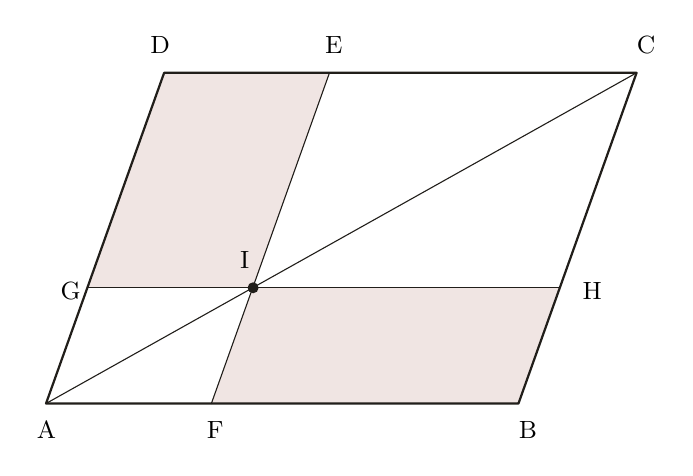
\begin{tikzpicture}[line cap=round,line join=round]
  \draw[fill=msred,fill opacity=0.13,draw=none] (2.70,0.66) -- (6.60,0.66) -- (7.13,2.13) -- (3.23,2.13) -- cycle;
  \draw[fill=msred,fill opacity=0.13,draw=none] (1.13,2.13) -- (3.23,2.13) -- (4.20,4.86) -- (2.10,4.86) -- cycle;
  \draw[msink,thick] (0.60,0.66) -- (6.60,0.66) -- (8.10,4.86) -- (2.10,4.86) -- cycle;
  \draw[msink] (0.60,0.66) -- (8.10,4.86);
  \draw[msink] (1.13,2.13) -- (7.13,2.13);
  \draw[msink] (2.70,0.66) -- (4.20,4.86);
  \fill[msink] (3.23,2.13) circle (0.07);
  \node[anchor=base west] at (0.36,0.21) {\small A};
  \node[anchor=base west] at (2.52,0.21) {\small F};
  \node[anchor=base west] at (6.48,0.21) {\small B};
  \node[anchor=base west] at (0.66,1.98) {\small G};
  \node[anchor=base west] at (2.94,2.37) {\small I};
  \node[anchor=base west] at (7.29,1.98) {\small H};
  \node[anchor=base west] at (1.80,5.10) {\small D};
  \node[anchor=base west] at (4.02,5.10) {\small E};
  \node[anchor=base west] at (7.98,5.10) {\small C};
\end{tikzpicture}
\mscaption{Redrawn after the marginal figure. The shaded figures are the two complements, FBHI and GIED.}
\end{msfigure}

\dutchtext{Bewijs mij, dat de Complimente\footnote{\textit{Complimente} --- the complements (Lat. \textit{complementa}) of a parallelogram: the two lesser parallelograms lying off the diagonal, one on either side of it, once the two parallelograms AFIG and IHCE about the diagonal are taken away.}, van Een parrallelogram FBHI, en GIED, Eeven groot, off\footnote{\textit{off} --- period spelling of \textit{of}, ``or''; \textit{Eeven groot}, ``equal in magnitude''. \textit{Exempel} is the reckoning-school term for a worked example, not an illustration.} aan malkander gelijk zijn.}
\engtext{Prove to me that the complements of a parallelogram, FBHI and GIED, are equal in magnitude, or equal to one another.}

\worktitle{Bewijs}{Proof}
\begin{workblock}
  \wrow{De}{$\triangle ABC = \triangle ADC$}{The diagonal AC halves the parallelogram.}
  \wrow{Substrh.\footnote{\textit{Substrh.} abbreviates \textit{substraheert}, ``subtract''. \textit{Komt}, literally ``there comes'', is the standard Dutch term for the outcome of an operation, as in a division or subtraction sum; the rule beneath the line is the sum's rule, not a fraction bar.}}{$\triangle IHC = \triangle IEC$}{Subtract the two triangles about the diagonal --- the halves of IHCE.}\ruleunder
  \wrow{komt}{$\square ABHI = \square ADEI$}{There remains ABHI = ADEI.}
  \wrow{De}{$\triangle AFI = \triangle AGI$}{Subtract likewise the halves of AFIG.}\ruleunder
  \wrow{komt}{$\square FBHI = \square GIED$}{The two complements are equal.}
  \wnote{'t welke te bewijse was.\footnote{\textit{'t welke te bewijse was} --- the Dutch rendering of \textit{quod erat demonstrandum}.} \textit{--- which was to be demonstrated.}}
\end{workblock}

\reading{The diagonal AC bisects the parallelogram ABCD, so $\triangle$ABC = $\triangle$ADC. Subtracting from these the triangles IHC and IEC --- equal to one another, being the halves of the small parallelogram IHCE about the diagonal --- leaves ABHI = ADEI. Subtracting further the equal triangles AFI and AGI, the halves of AFIG, leaves the two complements FBHI = GIED. The proposition is Euclid, \textit{Elements} I.43;\footnote{Euclid I.43: \textit{in any parallelogram the complements of the parallelograms about the diameter are equal to one another}. The scribe writes a leaning parallelogram glyph for the first two results and an upright rectangle for the last; both denote the same figures, and are set uniformly as $\square$ here.} the examiner reproduces it in the abbreviated reckoning-school layout, as a subtraction sum with the operator word set in the left margin.}

\begin{msnotes}
  \item[6.] The GLOBALISE transcription is machine-generated (Loghi HTR) and garbles the lettered figures: the complements appear as \texttt{F B H11} and \texttt{CIL:O}, the subtraction line as \texttt{\#AINC-AIEC}, and \textit{Bewijs} as \texttt{Berijs}. The manuscript itself reads cleanly; the text above is corrected against the scan. Lines here are given in reading order, not in the transcription's own order.
\end{msnotes}

\exempel{2de Exempel}{Second Example}

\begin{msfigure}
\begin{tikzpicture}[line cap=round,line join=round]
  \draw[msink,thick] (0.72,0.90) -- (4.44,0.90) -- (2.76,4.68) -- cycle;
  \draw[msink,thick] (4.44,0.90) -- (8.28,0.90);
  \draw[msink,dashed] (4.44,0.90) -- (6.48,4.62);
  % arc in the source figure, omitted: M 166 170 A 18 18 0 0 0 155 154
  \node[anchor=base west] at (0.48,0.42) {\small A};
  \node[anchor=base west] at (4.29,0.42) {\small B};
  \node[anchor=base west] at (8.16,0.42) {\small D};
  \node[anchor=base west] at (2.58,4.86) {\small C};
  \node[anchor=base west] at (6.54,4.80) {\small E};
\end{tikzpicture}
\mscaption{Redrawn after the marginal figure. The base is produced to D and BE is drawn parallel to AC; the exterior angle CBD is marked.\footnote{The manuscript draws BE as a broken line, its consistent way of marking a line added for the construction rather than given in the proposition; the same convention appears in the figures to the twelfth and the twenty-first examples.}}
\end{msfigure}

\dutchtext{Bewijs mij, dat in een driehoek ABC alle drie de hoeke te zaame genoomen, gelijk zijn aan twee regte hoeke,\footnote{\textit{2L} --- two right angles. The manuscript uses one glyph, L, both for ``angle'' when it stands before three letters ($\angle$ABC) and for ``right angle'' when it stands after a number; the reading is fixed by position alone. It is set here as $\angle$ and as L respectively.} off 180 graden.}
\engtext{Prove to me that in a triangle ABC all three angles taken together are equal to two right angles, or 180 degrees.}

\worktitle{Bewijs}{Proof}
\begin{workblock}
  \wrow{De}{$\angle ABC + \angle CBD = 2L$}{The two angles on the straight line ABD.}
  \wrow{}{$\angle CBD = \angle BAC + \angle ACB$}{The exterior angle, cut by BE into the two interior ones.\footnote{The rule beneath the line is again the reckoning-school rule of a substitution, not a fraction bar: the term above it is replaced by the term below in the line that follows.}}\ruleunder
  \wrow{derhalve is}{$\angle ABC + \angle BAC + \angle ACB = 2L \;\textit{ off } 180^{\circ}$}{The three angles of the triangle.}
\end{workblock}

\reading{Euclid, \textit{Elements} I.32, in three lines. Produce the base to D and draw BE parallel to AC. The angles ABC and CBD stand on a straight line and so make two right angles; and the exterior angle CBD is split by BE into two parts, equal to the two remote interior angles --- the one by alternate angles, the other by corresponding angles. Substituting gives the three angles of the triangle. The examiner writes down neither the parallel nor the two angle rules that justify the second line; the figure carries them, and a candidate is expected to read them off it.}

\begin{msnotes}
  \item[4.] \textit{Off} 180 \textit{graden} --- ``or 180 degrees''. Euclid never states the theorem in degrees; the navigation school does, because a degree is the unit its pupils will actually work in.
\end{msnotes}

\exempel{3de Exempel}{Third Example}

\begin{msfigure}
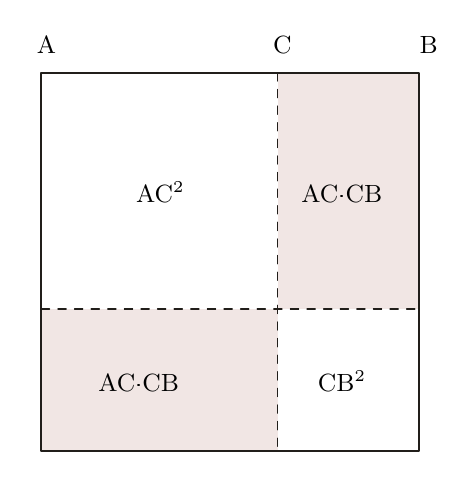
\begin{tikzpicture}[line cap=round,line join=round]
  \draw[fill=msred,fill opacity=0.12,draw=none] (4.20,2.70) rectangle (6.00,5.70);
  \draw[fill=msred,fill opacity=0.12,draw=none] (1.20,0.90) rectangle (4.20,2.70);
  \draw[msink,thick] (1.20,0.90) rectangle (6.00,5.70);
  \draw[msink,dashed] (4.20,5.70) -- (4.20,0.90);
  \draw[msink,dashed] (1.20,2.70) -- (6.00,2.70);
  \node[anchor=base west] at (1.02,5.94) {\small A};
  \node[anchor=base west] at (4.02,5.94) {\small C};
  \node[anchor=base west] at (5.88,5.94) {\small B};
  \node[anchor=base west] at (2.28,4.05) {\small AC$^{2}$};
  \node[anchor=base west] at (4.59,1.65) {\small CB$^{2}$};
  \node[anchor=base west] at (4.38,4.05) {\small AC\textperiodcentered{}CB};
  \node[anchor=base west] at (1.80,1.65) {\small AC\textperiodcentered{}CB};
\end{tikzpicture}
\mscaption{Redrawn after the marginal figure, which the manuscript draws in dotted lines and leaves unlettered within.\footnote{The four regions are named here for legibility; the manuscript leaves the square blank, marking only A, C and B along the top edge and drawing the interior divisions in dotted line. The proposition begins on this opening and its proof runs over on to the next (fol. 3600).}}
\end{msfigure}

\dutchtext{Bewijs mij, dat als Een regte lijn AB in Een punt C naar wilkeuren gedeeld is,\footnote{\textit{Naar wilkeuren} (modern \textit{naar willekeur}) --- ``at will'', arbitrarily; Euclid's \gk{ὡς} \gk{ἔτυχεν}. The point of the phrase is that the theorem holds for every division, which is what makes it worth proving.} dat het quadraet van de geheele lijn AB gelijk zij aan de beijde quadraaten van de deelen AC en CB, met twee maal den regthoek van deese deelen te zamen genoomen.\footnote{\textit{Den regthoek van deese deelen} --- the rectangle contained by the two parts, written $\square$AC,CB with a comma between the containing lines. \textit{Quadraet} is the square on a line, written as a raised 2 in the working but spelled out in the proposition.}}
\engtext{Prove to me that if a straight line AB is divided at will at a point C, the square on the whole line AB is equal to the two squares on the parts AC and CB, together with twice the rectangle contained by those parts.}

\worktitle{Bewijs}{Proof}
\begin{workblock}
  \wrow{}{$AB^2 = \square AB{,}AC + \square AB{,}BC$}{The whole square cut into two rectangles on the parts.}
  \wrow{}{$\square AB{,}AC = AC^2 + \square AC{,}BC$}{The first rectangle in its turn.}\ruleunder
  \wrow{derhalv. is}{$AB^2 = AC^2 + \square AB{,}BC + \square AC{,}CB$}{Substituting.}
  \wrow{en het}{$\square AB{,}BC = \square AC{,}CB + CB^2$}{And the second rectangle likewise.}\ruleunder
  \wrow{daarom}{$AB^2 = AC^2 + \square AC{,}BC + \square AC{,}CB + CB^2$}{All four pieces of the figure.}
  \wrow{dat is}{$AB^2 = AC^2 + 2\,\square AC{,}CB + BC^2$}{The two equal rectangles gathered into one term.}
  \wnote{dat het bewijse was. \textit{--- which was the thing to be proved.}}
\end{workblock}

\reading{Euclid, \textit{Elements} II.4 --- in modern notation (a + b)$^{2}$ = a$^{2}$ + 2ab + b$^{2}$, though the manuscript has no notion of an algebraic identity and none of a general a and b. Everything is a figure: the square on AB really is a square, cut by two lines through C into a square on AC, a square on CB, and two equal rectangles on AC and CB. The proof dissects it twice over, first splitting the whole square into two rectangles, then splitting each of those, and finally gathers the two equal rectangles into the single term ``2 $\square$AC,CB''. The examination sets this and the two following examples as a group: II.4, II.5 and II.6 in Euclid's order, the standard sequence of the second book.}

\begin{msnotes}
  \item[4.] The machine transcription of the proof is unusable --- \texttt{ABE HAB, ACtGAB, BC} for the first line and \texttt{datis A8 AC't2AC, CBt BC} for the last. The $\square$ glyph is read as a letter throughout. All readings taken from the scan.
\end{msnotes}

\foliomark{3600}{0033}{4--6}

\foliostand{The second book of Euclid \textperiodcentered{} cutting a line and squaring the parts}{The sixth example's proof stands on the next opening; it is given here with its proposition.}

\exempel{4de Exempel}{Fourth Example}

\begin{msfigure}
\begin{tikzpicture}[line cap=round,line join=round]
  \draw[msink,thick] (0.60,4.98) -- (6.90,4.98);
  \draw[msink] (0.60,5.16) -- (0.60,4.80);
  \draw[msink] (3.75,5.16) -- (3.75,4.80);
  \draw[msink] (5.01,5.16) -- (5.01,4.80);
  \draw[msink] (6.90,5.16) -- (6.90,4.80);
  % arc in the source figure, omitted: M 167 60 L 230 60 L 230 165 L 125 165 L 125 102 L 
  \draw[msink,thick] (3.75,1.05) rectangle (6.90,4.20);
  \draw[msink,dashed] (5.01,4.20) -- (5.01,1.05);
  \draw[msink,dashed] (3.75,2.94) -- (6.90,2.94);
  \node[anchor=base west] at (0.45,5.34) {\small A};
  \node[anchor=base west] at (3.60,5.34) {\small C};
  \node[anchor=base west] at (4.86,5.34) {\small D};
  \node[anchor=base west] at (6.75,5.34) {\small B};
  \node[anchor=base west] at (3.90,3.42) {\small CD$^{2}$};
  \node[anchor=base west] at (5.28,1.80) {\small AD\textperiodcentered{}DB};
\end{tikzpicture}
\mscaption{Redrawn after the marginal figure. The shaded gnomon is the rectangle AD\textperiodcentered{}DB; the small square is CD$^{2}$.\footnote{The regions are named here for legibility. The manuscript draws the figure in dotted line at the head of the example and letters only A, C, D and B along the top edge, leaving the reader to identify the parts from the working.}}
\end{msfigure}

\dutchtext{Om te bewijsen, dat als Een Regte lijn AB in twee gelijke deele gedeelt worde in C, en in twee ongelijke deelen in D, zal de regthoek van de ongelijke deele AD en DB, met het quadraat van het middelstuk der deelinge CD\footnote{\textit{Het middelstuk der deelinge} --- ``the middle piece of the division'', CD, the interval between the point of equal section and the point of unequal section. \textit{Halfscheid} (modern \textit{helft}) is the half.} te zamen genoomen, aan het quadraat van de halfscheid CB der gedeelde lijn AB gelijk zijn.}
\engtext{To prove that if a straight line AB is divided into two equal parts at C and into two unequal parts at D, the rectangle contained by the unequal parts AD and DB, together with the square on the middle piece of the division CD, is equal to the square on the half CB of the divided line AB.}

\worktitle{Bewijs}{Proof}
\begin{workblock}
  \wrow{}{$CB^2 = \square CB{,}BD + \square CB{,}CD$}{The square on the half, cut by D into two rectangles.}
  \wrow{en}{$\square CB{,}CD = \square CD{,}BD + CD^2$}{And the second of them cut again.}\ruleunder
  \wrow{derhalv. is}{$CB^2 = \square CB{,}BD + \square CD{,}BD + CD^2$}{Substituting.}
  \wrow{dan is het}{$\square \underline{AC}{,}BD + \square CD{,}BD = \square AD{,}BD$}{CB written as AC, its equal, so that AC and CD compose AD.\footnote{The manuscript marks the substitution with a double rule under AC, its habitual sign that a term is being exchanged for its equal --- here CB for AC, the two halves of the bisected line. The underline is reproduced.}}\ruleunder
  \wrow{daarom}{$CB^2 = \square AD{,}BD + CD^2$}{The proposition.}
  \wnote{dat te bewijse was. \textit{--- which was to be proved.}}
\end{workblock}

\reading{Euclid, \textit{Elements} II.5 --- the proposition that the mean of two numbers exceeds their geometric mean, though nobody in 1787 would have put it that way. The method is the same dissection as in the third example, worked in the other direction: the square on the half is broken into two rectangles, one of those into a rectangle and a square, and the two rectangles standing on BD are then gathered into one on AD. The whole argument is four substitutions, each licensed by the figure and none by a stated axiom.}

\begin{msnotes}
  \item[4.] The machine transcription of this proof is unusable --- \texttt{cBEDES, BDtHEB, CO} for the first line, \texttt{HACBDTGCDBO-AD B0} for the fourth. The $\square$ glyph is consistently read as a letter. All readings taken from the scan.
\end{msnotes}

\exempel{5de Exempel}{Fifth Example}

\begin{msfigure}
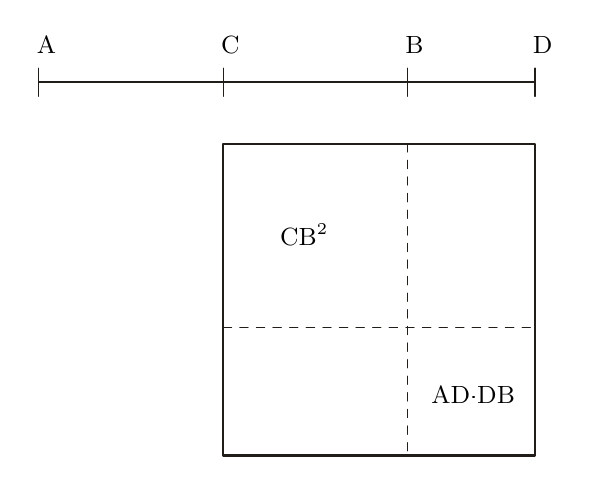
\begin{tikzpicture}[line cap=round,line join=round]
  \draw[msink,thick] (0.60,4.98) -- (6.90,4.98);
  \draw[msink] (0.60,5.16) -- (0.60,4.80);
  \draw[msink] (2.94,5.16) -- (2.94,4.80);
  \draw[msink] (5.28,5.16) -- (5.28,4.80);
  \draw[msink] (6.90,5.16) -- (6.90,4.80);
  % arc in the source figure, omitted: M 176 60 L 230 60 L 230 192 L 98 192 L 98 138 L 17
  \draw[msink,thick] (2.94,0.24) rectangle (6.90,4.20);
  \draw[msink,dashed] (5.28,4.20) -- (5.28,0.24);
  \draw[msink,dashed] (2.94,1.86) -- (6.90,1.86);
  \node[anchor=base west] at (0.45,5.34) {\small A};
  \node[anchor=base west] at (2.79,5.34) {\small C};
  \node[anchor=base west] at (5.13,5.34) {\small B};
  \node[anchor=base west] at (6.75,5.34) {\small D};
  \node[anchor=base west] at (3.54,2.91) {\small CB$^{2}$};
  \node[anchor=base west] at (5.46,0.90) {\small AD\textperiodcentered{}DB};
\end{tikzpicture}
\mscaption{Redrawn after the marginal figure. AB is bisected at C and produced to D; the shaded gnomon is AD\textperiodcentered{}DB.}
\end{msfigure}

\dutchtext{Bewijst mij, dat als Een regte lijn AB midde door gedeelt word in C, en vervolgens verlengt tot Eenig bepaald punt D, zal de regthoek die de geheelen lijn AB met het aangevoegde stuk BD te zaamen tot Lengte heeft, en het aangevoegde stuk alleen tot Breete,\footnote{The proposition is stated the long way round --- a rectangle described by naming its length and its breadth in turn --- rather than as ``the rectangle contained by AD and DB''. This is the schoolroom formula, meant to be read aloud and reconstructed on a slate; the working then abbreviates it at once to $\square$AD,BD.} met het quadraat CB der halve gedeelde lijn AB te zaamen genoomen, aan 't quadraat gelijk zijn dat op de helfte CB der gedeelde lijn met het aangevoegde stuk BD als Een regte lijn CD beschreeven is.}
\engtext{Prove to me that if a straight line AB is bisected at C and then produced to any given point D, the rectangle having for its length the whole line AB together with the added piece BD, and for its breadth the added piece alone, taken together with the square on the half CB of the divided line, is equal to the square described on CD --- that is, on the half CB together with the added piece BD taken as one straight line.}

\worktitle{Bewijs}{Proof}
\begin{workblock}
  \wrow{}{$CD^2 = \square CD{,}CB + \square CD{,}BD$}{The square on CD cut at B into two rectangles.}
  \wrow{}{$\square CD{,}CB = \square CB{,}BD + CB^2$}{The first of them cut again.}\ruleunder
  \wrow{derhalve is}{$CD^2 = \square CB{,}BD + \square CD{,}BD + CB^2$}{Substituting.}
  \wrow{}{$\square \underline{AC}{,}BD + \square CD{,}BD = \square AD{,}BD$}{CB again written as AC, so that the two rectangles gather onto AD.}\ruleunder
  \wrow{daerom is}{$CD^2 = \square AD{,}DB + BC^2$}{The proposition.}
  \wnote{het welke te bewijsen was.}
\end{workblock}

\reading{Euclid, \textit{Elements} II.6 --- the companion to the fourth example, and the one Euclid uses to justify the construction of II.11 that the tenth example will need. The two propositions are the same dissection with the point D taken inside the line in one case and outside it in the other, and the examiner's working is line for line the same, down to the substitution of AC for CB. The examination is testing whether a candidate sees that they are one proposition in two positions.}

\begin{msnotes}
  \item[2.] \textit{Aangevoegde stuk} --- the added piece, BD, by which the line is produced beyond B; \textit{beschreeven}, described, of a square erected on a line.
  \item[3.] The hand alternates freely between BC and CB, and between DB and BD, within a single line of working; the order of the letters carries no meaning for a rectangle or a square. The manuscript's own order is kept here.
\end{msnotes}

\exempel{6de Exempel}{Sixth Example}

\begin{msfigure}
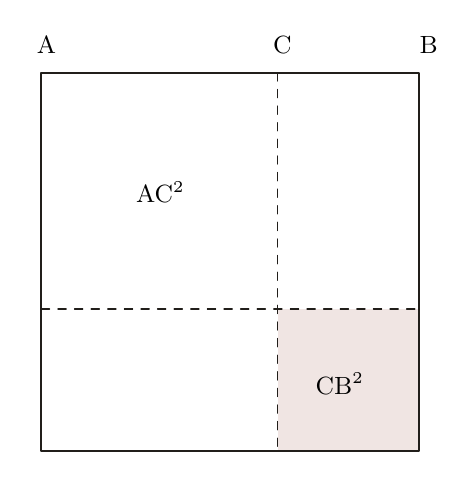
\begin{tikzpicture}[line cap=round,line join=round]
  \draw[fill=msred,fill opacity=0.13,draw=none] (4.20,0.90) rectangle (6.00,2.70);
  \draw[msink,thick] (1.20,0.90) rectangle (6.00,5.70);
  \draw[msink,dashed] (4.20,5.70) -- (4.20,0.90);
  \draw[msink,dashed] (1.20,2.70) -- (6.00,2.70);
  \node[anchor=base west] at (1.02,5.94) {\small A};
  \node[anchor=base west] at (4.02,5.94) {\small C};
  \node[anchor=base west] at (5.88,5.94) {\small B};
  \node[anchor=base west] at (2.28,4.05) {\small AC$^{2}$};
  \node[anchor=base west] at (4.56,1.62) {\small CB$^{2}$};
\end{tikzpicture}
\mscaption{The same divided square as the third example, put to a different account.\footnote{The manuscript draws a fresh figure at the head of the example, but it is the same divided square as the third --- evidence that the examiner is working from a set of standard diagrams rather than constructing each afresh. The proof, in the event, does not use it at all.}}
\end{msfigure}

\dutchtext{Om te bewijsen, dat als Een regte lijn AB in Een punt C naar welgevalle gedeelt word, dat de twee regthoeke die beijde de Lengte der geheele lijn AB en de Breete van Een der deele BC hebben, met het quadraat van het andere deel AC te zamen, gelijk aan het quadraat van de geheele lijn AB met het quadraat van het Eerste genoomen deel CB te zaamen genoomen is.}
\engtext{To prove that if a straight line AB is divided at pleasure at a point C, the two rectangles having both the length of the whole line AB and the breadth of one of the parts BC, together with the square on the other part AC, are equal to the square on the whole line AB together with the square on the part first taken, CB.}

\worktitle{Bewijs}{Proof}
\begin{workblock}
  \wnote{{\color{msmut}\small fol. 3601}}
  \wrow{}{$AB^2 = AC^2 + 2\,\square AC{,}CB + CB^2$}{The third example, taken as already proved.}
  \wrow{en}{$CB^2 \qquad\qquad CB^2 \textit{ bij gevoegt}$}{The same square added to both sides.\footnote{\textit{Bij gevoegt} --- ``added to'', the fourth of the operator words the paper uses beside \textit{substraheert}, \textit{trekt … aff} and \textit{adeert}. The line is written with CB$^{2}$ standing alone on both sides of the page and a rule beneath, the reckoning-school way of showing an addition made to both members of an equation at once.}}\ruleunder
  \wrow{komt}{$AB^2 + CB^2 = AC^2 + 2\,\square AC{,}CB + 2\,CB^2$}{The left side is now the sum the proposition names.}
  \wrow{}{$2\,\square AC{,}CB + 2\,CB^2 = 2\,\square AB{,}BC$}{Because AC and CB together make AB.}\ruleunder
  \wrow{derhalve is}{$AB^2 + CB^2 = AC^2 + 2\,\square AB{,}BC$}{The proposition.}
  \wnote{'t welk te bewijsen was.}
\end{workblock}

\reading{Euclid, \textit{Elements} II.7, and the first example on the paper that is proved from an earlier one rather than from the figure. The examiner takes the third example's result as given, adds CB$^{2}$ to both sides, and observes that 2 AC\textperiodcentered{}CB + 2 CB$^{2}$ is 2 AB\textperiodcentered{}BC --- which is true because AC + CB is AB, and is the one step that the figure alone will not hand him. It marks a change of method: from here to the ninth example the proofs build on one another, and the examination is testing the sequence, not the individual dissections.}

\begin{msnotes}
  \item[2.] \textit{Het werk volgt} is the manuscript's own catchword for a proof continued over the page; it recurs at the ninth example, whose proof stands two openings later. The proof is set here with its proposition, its folio noted; the examples, not the folios, are the units of this edition.
\end{msnotes}

\foliomark{3601}{0034}{7--9}

\foliostand{The obtuse and acute triangle \textperiodcentered{} and the diagonals of a parallelogram}{The ninth example's working stands two openings later; it is given here with its proposition.}

\exempel{7de Exempel}{Seventh Example}

\begin{msfigure}
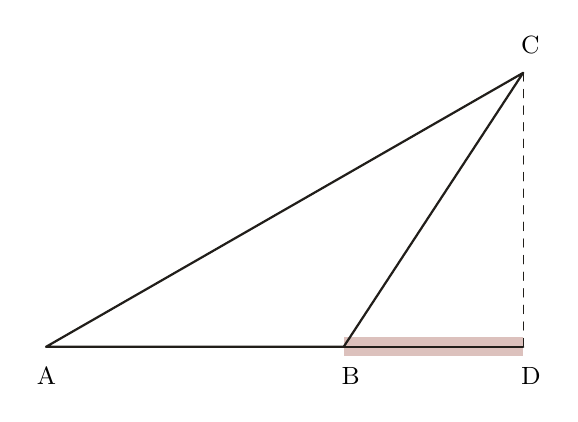
\begin{tikzpicture}[line cap=round,line join=round]
  \draw[fill=msred,fill opacity=0.3,draw=none] (4.50,0.84) rectangle (6.78,1.08);
  \draw[msink,thick] (0.72,0.96) -- (4.50,0.96) -- (6.78,4.44) -- cycle;
  \draw[msink,thick] (4.50,0.96) -- (6.78,0.96);
  \draw[msink,dashed] (6.78,4.44) -- (6.78,0.96);
  % arc in the source figure, omitted: M 226 156 L 214 156 L 214 168
  \node[anchor=base west] at (0.48,0.48) {\small A};
  \node[anchor=base west] at (4.35,0.48) {\small B};
  \node[anchor=base west] at (6.63,0.48) {\small D};
  \node[anchor=base west] at (6.63,4.68) {\small C};
\end{tikzpicture}
\mscaption{Redrawn after the marginal figure. The angle at B is obtuse, so the perpendicular CD falls outside the base; BD is the shaded piece.}
\end{msfigure}

\dutchtext{Om te bewijsen, dat van Een stompehoekige driehoek ABC het quadraat der zijde AC over den stompe hoek ABC,\footnote{\textit{Over den stompe hoek} --- ``over'', that is opposite to, the obtuse angle; the eighth example has \textit{teegen over} in the same sense. \textit{Stompehoekig}, obtuse-angled; \textit{scherpe hoek}, acute angle.} gelijk aan de Som der quadraaten van de Basis AB en van de anderen zijde BC te samen genoomen met twee regthoeke die de Lengte der Basis hebben en de Breete van het verlengde stuk der Basis, dat tusschen de stompe hoek ABC en den perpendiculaar CD, die uijt den top hoek C op de verlengde Basis valt, bevat is.}
\engtext{To prove that in an obtuse-angled triangle ABC the square on the side AC subtending the obtuse angle ABC is equal to the sum of the squares on the base AB and on the other side BC, taken together with two rectangles having the length of the base and the breadth of that produced piece of the base contained between the obtuse angle ABC and the perpendicular CD let fall from the vertex C upon the base produced.}

\worktitle{Bewijs}{Proof}
\begin{workblock}
  \wrow{}{$AC^2 = AD^2 + DC^2$}{Pythagoras on the right triangle ADC.}
  \wrow{}{$AD^2 = AB^2 + 2\,\square AB{,}BD + BD^2$}{The third example applied to AD, cut at B.}\ruleunder
  \wrow{derh.}{$AC^2 = AB^2 + 2\,\square AB{,}BD + BD^2 + DC^2$}{Substituting.}
  \wrow{en}{$BD^2 + DC^2 = BC^2$}{Pythagoras again, on the small right triangle BDC.}\ruleunder
  \wrow{daarom}{$AC^2 = AB^2 + BC^2 + 2\,\square AB{,}BD$}{The proposition.}
  \wnote{dat te bewijsen was.}
\end{workblock}

\reading{Euclid, \textit{Elements} II.12 --- the obtuse case of what is now the law of cosines, the excess over Pythagoras being twice the rectangle on the base and the projection. The examiner proves it in four lines by taking Pythagoras twice and the third example once, and the manuscript's method has now completely settled into this shape: cite an earlier result, substitute, cite another, substitute again. No figure is argued from; the diagram serves only to name the letters.}

\begin{msnotes}
  \item[2.] The proposition names the excess as ``two rectangles having the length of the base and the breadth of the produced piece'' --- that is, 2 AB\textperiodcentered{}BD --- rather than as twice one rectangle. The working writes it 2 $\square$AB,BD at once.
  \item[3.] Pythagoras is used twice without being cited; it is proved as the fifteenth example, eight propositions later on the paper. The order is the examination's, not a deductive one --- a candidate is expected to have the theorem in hand long before he is asked to demonstrate it.
\end{msnotes}

\exempel{8de Exempel}{Eighth Example}

\begin{msfigure}
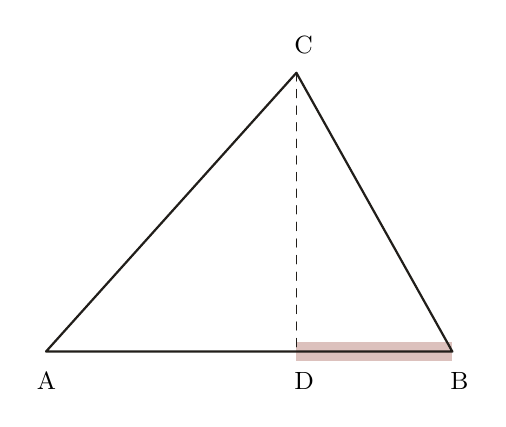
\begin{tikzpicture}[line cap=round,line join=round]
  \draw[fill=msred,fill opacity=0.3,draw=none] (3.90,0.84) rectangle (5.88,1.08);
  \draw[msink,thick] (0.72,0.96) -- (5.88,0.96) -- (3.90,4.50) -- cycle;
  \draw[msink,dashed] (3.90,4.50) -- (3.90,0.96);
  % arc in the source figure, omitted: M 130 156 L 142 156 L 142 168
  \node[anchor=base west] at (0.48,0.48) {\small A};
  \node[anchor=base west] at (3.75,0.48) {\small D};
  \node[anchor=base west] at (5.73,0.48) {\small B};
  \node[anchor=base west] at (3.75,4.74) {\small C};
\end{tikzpicture}
\mscaption{Redrawn after the marginal figure. The angle at B is acute, so the perpendicular falls within the base; BD is the shaded piece.}
\end{msfigure}

\dutchtext{Om te bewijsen, dat in ieder driehoek ABC het quadraat der zijde AC, die teegen over een scherpe hoek ABC staadt, gelijk aan de som der quadraaten van de basis AB en van de overige zijden BC te samen genoomen, min twee regthoeken\footnote{\textit{Min} --- ``less'', the only subtraction in any of the propositions as stated. Euclid's II.13 is likewise the one proposition of the second book whose enunciation subtracts rather than adds.} die de Lengte der Basis AB hebben en de breete van der zelver deel BD, dat tusschen den scherpenhoek ABC en der perpendiculaar, die uijt den top hoek op de Basis valt, bevat is.}
\engtext{To prove that in any triangle ABC the square on the side AC standing opposite an acute angle ABC is equal to the sum of the squares on the base AB and on the remaining side BC, less two rectangles having the length of the base AB and the breadth of that part of it, BD, contained between the acute angle ABC and the perpendicular let fall from the vertex upon the base.}

\worktitle{Bewijs}{Proof}
\begin{workblock}
  \wrow{}{$2\,\square AB{,}BD + AD^2 = AB^2 + BD^2$}{The sixth example, on AB cut at D.\footnote{The first line is the sixth example (Euclid II.7) with AB cut at D instead of at C; the examiner does not say so, writing it down as a known result. This is the only place on the paper where an earlier example is re-lettered before use.}}
  \wrow{Addeert}{$DC^2 \qquad\qquad DC^2$}{The same square added to both members.}\ruleunder
  \wrow{komt}{$2\,\square AB{,}BD + \underline{AD^2 + DC^2} = AB^2 + \underline{BD^2 + DC^2}$}{Both underlined pairs are hypotenuses by Pythagoras.\footnote{The manuscript double-underlines AD$^{2}$ + DC$^{2}$ and BD$^{2}$ + DC$^{2}$ in the third line --- its standing mark for a group about to be replaced by its equal. The underlines are reproduced here.}}
  \wrow{dat is}{$2\,\square AB{,}BD + AC^2 = AB^2 + BC^2$}{The proposition, with the rectangles brought to the other side.}
  \wnote{'t geen te bewijsen was.}
\end{workblock}

\reading{Euclid, \textit{Elements} II.13, the acute case, and the pair to the example before it. The examiner's working is elegant here: adding DC$^{2}$ to both members of the sixth example turns AD$^{2}$ + DC$^{2}$ into AC$^{2}$ on one side and BD$^{2}$ + DC$^{2}$ into BC$^{2}$ on the other, and the proposition falls out in a single stroke. He states the result in the additive form, with the two rectangles standing on the left beside AC$^{2}$, rather than as a subtraction --- although the proposition itself is worded with \textit{min}, less. The two forms are the same statement.}

\begin{msnotes}
  \item[4.] The closing formula is written \textit{'t geen te bewijsen} with \textit{was} squeezed in below the line, the hand having run out of room at the edge of the leaf.
\end{msnotes}

\exempel{9de Exempel}{Ninth Example}

\begin{msfigure}
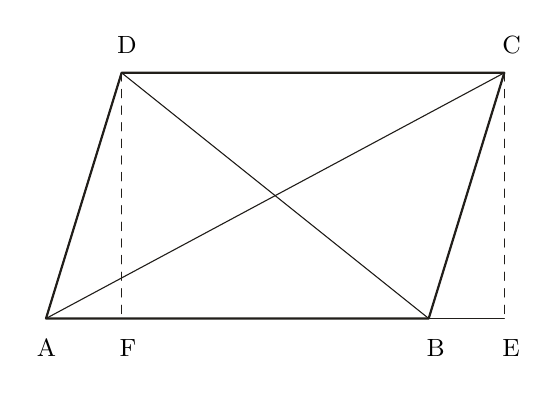
\begin{tikzpicture}[line cap=round,line join=round]
  \draw[msink] (1.02,1.08) -- (6.84,4.20);
  \draw[msink] (5.88,1.08) -- (1.98,4.20);
  \draw[msink,thick] (1.02,1.08) -- (5.88,1.08) -- (6.84,4.20) -- (1.98,4.20) -- cycle;
  \draw[msink] (5.88,1.08) -- (6.84,1.08);
  \draw[msink,dashed] (1.98,4.20) -- (1.98,1.08);
  \draw[msink,dashed] (6.84,4.20) -- (6.84,1.08);
  \node[anchor=base west] at (0.78,0.60) {\small A};
  \node[anchor=base west] at (1.83,0.60) {\small F};
  \node[anchor=base west] at (5.73,0.60) {\small B};
  \node[anchor=base west] at (6.69,0.60) {\small E};
  \node[anchor=base west] at (1.80,4.44) {\small D};
  \node[anchor=base west] at (6.69,4.44) {\small C};
\end{tikzpicture}
\mscaption{Redrawn after the marginal figure. The diagonals are marked; DF falls within the base, CE upon it produced.\footnote{The manuscript letters the figure D and C above, F, B and E below, with A at the left-hand corner of the leaf; the perpendiculars DF and CE are in dotted line. The two diagonals are drawn solid and are picked out here in the accent colour.}}
\end{msfigure}

\dutchtext{Om te bewijsen, als in een Parallellogram ABCD de beijde diagonale AC en BD worden getrokken, dat de som der quadraaten deezer beijde diagonale gelijk zijn aan de som der quadraate van alle vier de zijde van het Parallellogram.}
\engtext{To prove that if in a parallelogram ABCD both diagonals AC and BD are drawn, the sum of the squares on these two diagonals is equal to the sum of the squares on all four sides of the parallelogram.}

\worktitle{Bewijs}{Proof}
\begin{workblock}
  \wnote{{\color{msmut}\small fol. 3602}}
  \wrow{}{$AC^2 = AB^2 + BC^2 + 2\,\square AB{,}BE$}{The seventh example: the angle ABC is obtuse.}
  \wrow{en}{$BD^2 = AB^2 + AD^2 - 2\,\square AB{,}AF$}{The eighth: the angle DAB is acute.\footnote{The manuscript writes this line with a minus sign, the only one on the paper. It is the eighth example in its subtractive form, the form in which that proposition was enunciated but not the form in which it was concluded.}}\ruleunder
  \wrow{komt}{$AC^2 + BD^2 = AB^2 + BC^2 + AB^2 + AD^2$}{The two rectangles are equal and destroy one another.\footnote{That 2 $\square$AB,BE and 2 $\square$AB,AF are equal --- the projections of BC and AD upon AB, which are equal sides --- is nowhere stated; the examiner simply drops both terms in passing to the third line. It is the one real gap in an otherwise complete argument.}}
  \wrow{}{$AB^2 = DC^2$}{One of the two AB$^{2}$ written as the opposite side it equals.}\ruleunder
  \wrow{derhalves}{$AC^2 + BD^2 = AB^2 + BC^2 + DC^2 + AD^2$}{All four sides of the parallelogram.}
  \wnote{'t welk te bewijse was.}
\end{workblock}

\reading{The parallelogram law, and the summit of this part of the examination: it is the one proposition here that Euclid's second book does not contain, and it is proved by using the seventh and eighth examples together --- the obtuse case for one diagonal, the acute case for the other. The two correction rectangles are equal, since AF and BE are the projections of the two equal opposite sides, so they cancel; what is left is four squares, and the last substitution turns the repeated AB$^{2}$ into DC$^{2}$ so that the four are the four sides. Nine examples have built to this in a single unbroken chain, and having reached it the paper turns away from proof altogether: the tenth example is a construction.}

\begin{msnotes}
  \item[4.] The machine transcription of this proof is among the worst on the paper --- \texttt{ACE ABTECtEnAB,EE} for the first line, \texttt{der halvis Ac't B0s 48\#Bct Dc 440} for the last. All readings taken from the scan.
\end{msnotes}

\foliomark{3602}{0035}{10--12}

\foliostand{Examination of 28 November 1787 \textperiodcentered{} one opening, three propositions}{Each example is given a page of its own; the manuscript sets three to the opening.}

\exempel{10de Exempel}{Tenth Example}

\begin{msfigure}
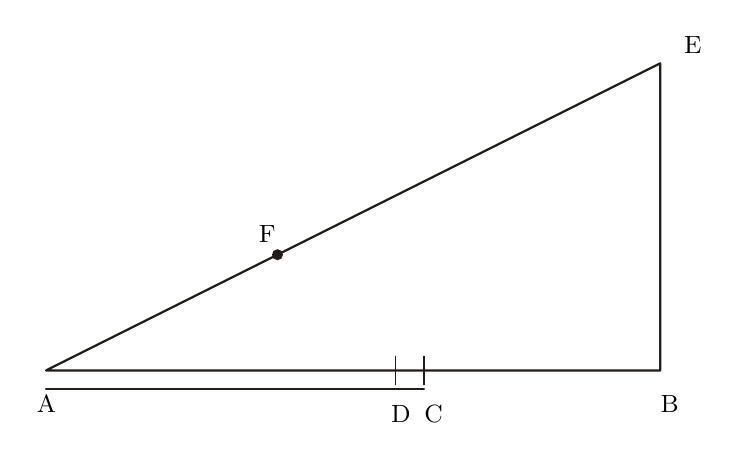
\begin{tikzpicture}[line cap=round,line join=round]
  \draw[msink,thick] (0.60,0.90) -- (8.40,0.90) -- (8.40,4.80) -- cycle;
  % arc in the source figure, omitted: M 268 170 L 268 158 L 280 158
  \draw[msink,thick] (0.60,0.66) -- (5.40,0.66);
  \draw[msink] (5.40,1.08) -- (5.40,0.72);
  \draw[msink] (5.04,1.08) -- (5.04,0.72);
  \fill[msink] (3.54,2.37) circle (0.07);
  \node[anchor=base west] at (0.36,0.36) {\small A};
  \node[anchor=base west] at (4.86,0.24) {\small D};
  \node[anchor=base west] at (5.28,0.24) {\small C};
  \node[anchor=base west] at (8.28,0.36) {\small B};
  \node[anchor=base west] at (8.58,4.92) {\small E};
  \node[anchor=base west] at (3.18,2.52) {\small F};
\end{tikzpicture}
\mscaption{Redrawn after the marginal sketch. BE is half of AB; F is cut off on AE by EF = EB; AC is set equal to AF.\footnote{The marginal sketch also carries a point D on AB, immediately to the left of C. It plays no part in the written proof and is left unlabelled in the argument; it is probably the corner of the square on AB that the standard construction erects and that the examiner has here dispensed with.}}
\end{msfigure}

\dutchtext{Om een regte lijn AB, in een punt C, zoodaanig te deelen, dat de regthoek, die de Lengte van de geheele lijn AB, en de Breete van het klijnste stuk CB heeft, gelijk zij aan het quadraat van het groote stuk AC; als meede met het zelvige Bewijs.\footnote{\textit{Regthoek} here is not ``right angle'' but the \textit{rectangle contained by} two lines, in the Euclidean sense --- its ``Lengte'' and ``Breete'' are the two lines named. \textit{Quadraat} is the square on a line. \textit{Als meede met het zelvige Bewijs} --- ``and likewise with the proof of the same'' --- is the examiner's formula requiring the demonstration and not merely the construction.}}
\engtext{To divide a straight line AB at a point C in such a way that the rectangle having the length of the whole line AB and the breadth of the lesser part CB is equal to the square on the greater part AC; together with the proof of the same.}

\worktitle{Bewijs}{Proof}
\begin{workblock}
  \wrow{}{$AE^2 = AB^2 + BE^2$}{The right angle stands at B.}
  \wrow{en}{$AE^2 = EF^2 + 2\,EF\!\cdot\!AF + AF^2$}{AE is cut at F, so the square on it is the square on the two parts.}\ruleunder
  \wrow{derhalve is}{$\cancel{EF^2} + 2\,\cancel{EF}\!\times\!\cancel{AF} + \cancel{AF^2} = AB^2 + BE^2$}{The scribe double-underlines the terms he is about to replace: EF = BE, and AF = AC.\footnote{The manuscript marks substitution by a double rule beneath a term rather than by rewriting it: EF$^{2}$, EF, AF and AF$^{2}$ each carry one. The cancellation bars set here stand for those double rules. In the following line the terms have become AB$\times$AC and AC$^{2}$, BE$^{2}$ having fallen out on both sides.}}
  \wrow{dat is}{$AB\!\times\!AC + AC^2 = AB^2$}{Since 2 BE = AB.}
  \wrow{En}{$AB^2 = AB\!\times\!AC + AB\!\times\!BC$}{The whole square resolved on the two segments.}\ruleunder
  \wrow{daarom}{$AB\!\times\!AC + AC^2 = AB\!\times\!AC + AB\!\times\!BC$}{Both are equal to AB$^{2}$.}
  \wrow{trekt}{$AB\!\times\!AC = AB\!\times\!AC \quad \textit{aff}$}{``Take away'': \textit{trekt … aff}, the operator split around its object.\footnote{\textit{Trekt … aff} (modern \textit{trekt … af}), the separable verb of the reckoning schools for subtraction, exactly as \textit{substraheert} is used on the earlier examples; \textit{komt} introduces the result. The rule drawn beneath is the sum's rule, not a fraction bar.}}\ruleunder
  \wrow{komt}{$AC^2 = AB\!\times\!BC$}{Which is the section sought.}
  \wnote{dat te bewijsen was. \textit{--- which was to be proved.}}
\end{workblock}

\reading{This is the section of a line in extreme and mean ratio --- Euclid, \textit{Elements} II.11. The examiner does not argue from figures but from the algebra of the construction: erect BE equal to half of AB at right angles to it, join AE, cut off FE equal to BE, and set AC equal to AF. Then AE$^{2}$ is on one hand AB$^{2}$ + BE$^{2}$, and on the other the square on AF + FE; equating them and striking out the common BE$^{2}$ leaves AB$\times$AC + AC$^{2}$ = AB$^{2}$, and subtracting AB$\times$AC from the two expressions of AB$^{2}$ leaves AC$^{2}$ = AB$\times$BC. The ratio AC : AB is the golden section, 0\textperiodcentered{}618…, though the manuscript names no such thing.}

\exempel{11de Exempel}{Eleventh Example}

\begin{msfigure}
\begin{tikzpicture}[line cap=round,line join=round]
  \draw[msink,thick] (0.72,4.02) -- (8.28,4.02);
  \draw[msink,thick] (0.72,1.62) -- (8.28,1.62);
  \draw[msink] (2.10,0.42) -- (6.90,5.22);
  \draw[msink,dashed] (3.30,4.02) -- (3.30,1.62);
  \draw[msink,dashed] (5.70,4.02) -- (5.70,1.62);
  % arc in the source figure, omitted: M 208 66 A 18 18 0 0 1 177 79
  % arc in the source figure, omitted: M 112 146 A 18 18 0 0 1 143 133
  \node[anchor=base west] at (0.42,3.90) {\small R};
  \node[anchor=base west] at (3.12,4.26) {\small I};
  \node[anchor=base west] at (5.52,4.26) {\small G};
  \node[anchor=base west] at (8.40,3.90) {\small S};
  \node[anchor=base west] at (0.42,1.50) {\small T};
  \node[anchor=base west] at (3.12,1.14) {\small H};
  \node[anchor=base west] at (5.52,1.14) {\small K};
  \node[anchor=base west] at (8.40,1.50) {\small U};
  \node[anchor=base west] at (1.86,0.12) {\small N};
  \node[anchor=base west] at (6.90,5.34) {\small O};
  \node[anchor=base west] at (5.88,3.42) {\small u};
  \node[anchor=base west] at (3.78,1.80) {\small y};
\end{tikzpicture}
\mscaption{Redrawn after the marginal sketch. The dotted lines IH and GK are the perpendiculars; \textit{u} and \textit{y} are the alternate angles.}
\end{msfigure}

\dutchtext{Om te bewijsen, als twee Paralellijnen, RS en TU, van een derde lijn NO, in G, H doorsneeden worden, dat de overhandse Hoeken \textit{u} en \textit{y} aan malkander gelijk zijn.\footnote{\textit{Overhandse hoeken} --- literally ``over-hand angles'', the eighteenth-century Dutch term for alternate angles (modern \textit{verwisselende} or \textit{Z-hoeken}). \textit{Doorsneeden}, ``cut through''.}}
\engtext{To prove that when two parallel lines, RS and TU, are cut by a third line NO at G and H, the alternate angles \textit{u} and \textit{y} are equal to one another.}

\worktitle{Bewijs}{Proof}
\begin{workblock}
  \wrow{}{$\angle I = \angle K$}{Both are right, the two lines being perpendiculars.}
  \wrow{}{$HI = GK$}{The distance between two parallels is everywhere the same.}
  \wrow{}{$HG = HG$}{The common side.}\ruleunder
  \wrow{dan is}{$\triangle HGI = \triangle HGK$}{The two triangles are equal in every part.\footnote{The manuscript writes the congruence with a plain equals sign, as it does for equality of area throughout; the eighteenth century had no separate congruence symbol.}}
  \wrow{daarom is}{$\angle u = \angle y$}{The alternate angles are equal.\footnote{The congruence yields $\angle$IHG = $\angle$KGH. The marked angles exceed these by the right angles $\angle$IHT and $\angle$KGS respectively --- the perpendiculars standing at right angles to both parallels --- so \textit{u} and \textit{y} are themselves equal. The examiner leaves this last step unwritten.}}
  \wnote{het welk te bewijsen was. \textit{--- which was to be proved.}}
\end{workblock}

\reading{Euclid proves the equality of alternate angles by \textit{reductio} (Elements I.29); the examiner proves it by congruence instead. Drop the perpendicular IH from the upper parallel to the lower, and the perpendicular GK from the transversal's point on the upper line down to the lower --- both of the same length, since parallels stand everywhere the same distance apart. The triangles HGI and HGK then share the side HG and have equal right angles, and are therefore equal throughout, from which the alternate angles follow. This is a navigation-school proof: shorter than Euclid's, and resting on the equidistance of parallels rather than on the parallel postulate.}

\begin{msnotes}
  \item[4.] The machine transcription reads the proposition's figure letters as \texttt{25} and \texttt{T lb} for RS and TU, and renders \textit{$\triangle$HGI = $\triangle$HGK} as \texttt{AHI6I-AHICR}. Corrected against the scan.
\end{msnotes}

\exempel{12de Exempel}{Twelfth Example}

\begin{msfigure}
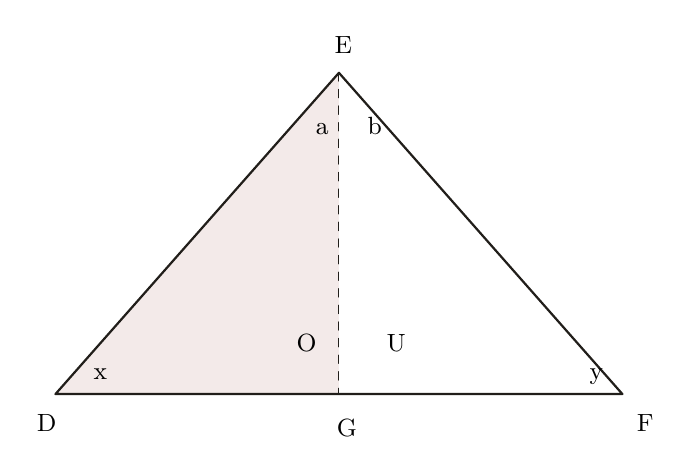
\begin{tikzpicture}[line cap=round,line join=round]
  \draw[fill=msred,fill opacity=0.10,draw=none] (4.50,5.04) -- (0.90,0.96) -- (4.50,0.96) -- cycle;
  \draw[msink,thick] (4.50,5.04) -- (0.90,0.96) -- (8.10,0.96) -- cycle;
  \draw[msink,dashed] (4.50,5.04) -- (4.50,0.96);
  % arc in the source figure, omitted: M 150 156 L 162 156 L 162 168
  % arc in the source figure, omitted: M 138 156 L 138 168
  \node[anchor=base west] at (4.32,5.28) {\small E};
  \node[anchor=base west] at (0.54,0.48) {\small D};
  \node[anchor=base west] at (4.35,0.42) {\small G};
  \node[anchor=base west] at (8.16,0.48) {\small F};
  \node[anchor=base west] at (4.08,4.26) {\small a};
  \node[anchor=base west] at (4.74,4.26) {\small b};
  \node[anchor=base west] at (1.26,1.14) {\small x};
  \node[anchor=base west] at (7.56,1.14) {\small y};
  \node[anchor=base west] at (3.84,1.50) {\small O};
  \node[anchor=base west] at (4.98,1.50) {\small U};
\end{tikzpicture}
\mscaption{Redrawn after the marginal sketch. EG is the perpendicular; the shaded half is the triangle DEG.}
\end{msfigure}

\dutchtext{Om te bewijsen, dat in een gelijkbeenige driehoek DEF, de hoeken aan de Basis \textit{x} en \textit{y} aan malkander gelijk zijn, en dat de perpendiculaar lijn EG, zo wel de hoek E ende Grondlijn DF, als de driehoek zelve, in twee gelijke deele deelt.\footnote{\textit{Gelijkbeenig}, ``equal-legged'', isosceles; \textit{grondlijn}, the base; \textit{perpendiculaar lijn}, the perpendicular --- a Latinism the Dutch schools kept beside the native \textit{loodlijn}. The proposition packs three conclusions into one statement, which is why the manuscript braces the three results together.}}
\engtext{To prove that in an isosceles triangle DEF the angles at the base, \textit{x} and \textit{y}, are equal to one another; and that the perpendicular EG divides the angle E, the base DF, and the triangle itself, each into two equal parts.}

\worktitle{Bewijs}{Proof}
\begin{workblock}
  \wrow{}{$DE = EF$}{Given: the triangle is \textit{gelijkbeenig}, equal-legged.}
  \wrow{}{$EG = EG$}{The common side.}
  \wrow{}{$\angle O = \angle U$}{The two angles at the foot G, both right.}\ruleunder
  \wrow{dan is de}{$\triangle DEG = \triangle GEF$}{Equal hypotenuse, common side, right angle.\footnote{The angles O and U are the two angles at G, right by construction. Strictly the congruence follows from the equal hypotenuses, the common side and the right angle; the examiner cites the three equalities in the order side--side--angle, as the schoolbooks then did.}}
  \wrow{daarom is}{$\angle a = \angle b$}{The apex angle is halved.}
  \wrow{}{$\angle x = \angle y$}{The base angles are equal.}
  \wrow{en}{$DG = GF$}{And the base is bisected.}
  \wnote{dat te bewijsen stond.\footnote{\textit{Dat te bewijsen stond} --- a variant of the closing formula used elsewhere on this page (\textit{dat te bewijsen was}, \textit{het welk te bewijsen was}). All three render \textit{quod erat demonstrandum}.} \textit{--- which stood to be proved.}}
\end{workblock}

\reading{Euclid's \textit{pons asinorum} (Elements I.5) proved by dropping the perpendicular: the two halves DEG and GEF have the equal legs DE and EF, the common EG, and the right angles at G, and are therefore equal in every part. Three conclusions follow at once, and the examiner braces them together as one: the apex angle is halved, the base angles are equal, and the base is bisected. The triangle is thereby divided into two equal parts as well --- the last clause of the proposition, which the proof establishes without stating it separately.}

\begin{msnotes}
  \item[4.] The machine transcription of this example is heavily corrupted --- \texttt{dan is de DOEb= DbEF} for \textit{$\triangle$DEG = $\triangle$GEF}, \texttt{1 N= 1 9} for $\angle$x = $\angle$y, and \texttt{O6= 6F} for DG = GF. All readings here are taken from the scan.
\end{msnotes}

\foliomark{3603}{0036}{13--15}

\foliostand{Equal parallelograms \textperiodcentered{} a construction \textperiodcentered{} and Pythagoras}{The one construction on the paper stands here, between two theorems.}

\exempel{13de Exempel}{Thirteenth Example}

\begin{msfigure}
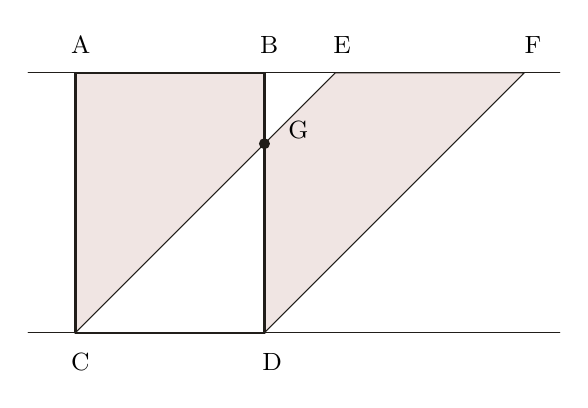
\begin{tikzpicture}[line cap=round,line join=round]
  \draw[fill=msred,fill opacity=0.13,draw=none] (1.20,4.50) -- (3.60,4.50) -- (3.60,3.60) -- (1.20,1.20) -- cycle;
  \draw[fill=msred,fill opacity=0.13,draw=none] (3.60,3.60) -- (4.50,4.50) -- (6.90,4.50) -- (3.60,1.20) -- cycle;
  \draw[msink] (0.60,4.50) -- (7.35,4.50);
  \draw[msink] (0.60,1.20) -- (7.35,1.20);
  \draw[msink,thick] (1.20,4.50) -- (3.60,4.50) -- (3.60,1.20) -- (1.20,1.20) -- cycle;
  \draw[msink] (4.50,4.50) -- (6.90,4.50) -- (3.60,1.20) -- (1.20,1.20) -- cycle;
  \fill[msink] (3.60,3.60) circle (0.07);
  \node[anchor=base west] at (1.02,4.74) {\small A};
  \node[anchor=base west] at (3.42,4.74) {\small B};
  \node[anchor=base west] at (4.35,4.74) {\small E};
  \node[anchor=base west] at (6.78,4.74) {\small F};
  \node[anchor=base west] at (1.02,0.72) {\small C};
  \node[anchor=base west] at (3.45,0.72) {\small D};
  \node[anchor=base west] at (3.78,3.66) {\small G};
\end{tikzpicture}
\mscaption{Redrawn after the marginal figure: both parallelograms stand on CD and between the same two parallels; G is where BD cuts CE.}
\end{msfigure}

\dutchtext{Om te bewijsen, dat twee parrallellograma ABCD en EFCD, gelijke Basis off grondlijn CD en gelijke hoogte AC hebbende,\footnote{\textit{Gelijke hoogte AC} --- the height is named by the side AC of the upright parallelogram, which serves as the perpendicular distance between the parallels. Euclid says instead that they are \textit{between the same parallels}; the figure here draws both lines and the examiner uses whichever formulation is nearer to hand.} aan malkander gelijk zijn.}
\engtext{To prove that two parallelograms ABCD and EFCD, having the same base or ground-line CD and the same height AC, are equal to one another.}

\worktitle{Bewijs}{Proof}
\begin{workblock}
  \wrow{}{$AB = CD$}{Opposite sides of the first parallelogram.}
  \wrow{en}{$CD = EF$}{And of the second.}\ruleunder
  \wrow{dan is ook}{$AB = EF$}{The two upper sides.}
  \wrow{addeert}{$BE = BE$}{The piece the two upper sides overlap upon.}\ruleunder
  \wrow{komt}{$AE = BF$}{The bases of the two end triangles.}
  \wrow{}{$AC = BD$}{The two heights.}
  \wrow{}{$CE = DF$}{The two slant sides.}\ruleunder
  \wrow{dan is}{$\triangle ACE = \triangle BDF$}{The two end triangles, equal in all three sides.}
  \wrow{subtr.}{$\triangle BEG = \triangle BEG$}{The small triangle the two overlap in.}\ruleunder
  \wrow{rest}{$\square ABGC = \square DFEG$}{Two four-sided pieces.\footnote{The manuscript writes the two quadrilaterals ABCG and DFEG, running the letters round the figure in whichever direction the eye takes them; the vertices are A, B, G, C and G, D, F, E. The $\square$ glyph is used here for four-sided pieces that are not parallelograms at all.}}
  \wrow{addeert}{$\triangle CGD = \triangle CGD$}{The triangle that completes each.}\ruleunder
  \wrow{komt}{$\square ABCD = \square EFCD$}{The two parallelograms.}
\end{workblock}

\reading{Euclid, \textit{Elements} I.35 --- parallelograms on the same base and between the same parallels are equal. This is the proposition on which the whole of Euclid's theory of area rests, and the first example on this paper proved it in the special case of the complements. The working is a single ledger of additions and subtractions: build the two end triangles equal, take away the piece they share, add back the piece that completes them, and the two parallelograms are left. The operator words are the reckoning-master's throughout --- \textit{addeert}, \textit{subtr.}, \textit{rest}, \textit{komt} --- applied to figures instead of numbers.}

\begin{msnotes}
  \item[3.] \textit{Rest} --- ``there remains'', the term for the residue of a subtraction, beside \textit{komt} for the result of an operation generally. Both are ordinary Dutch bookkeeping words.
\end{msnotes}

\exempel{14de Exempel}{Fourteenth Example}

\begin{msfigure}
\begin{tikzpicture}[line cap=round,line join=round]
  \draw[msink,thick] (0.60,1.05) -- (7.80,1.05);
  \draw[msink] (4.20,4.74) -- (2.10,1.05);
  \draw[msink] (4.20,4.74) -- (6.30,1.05);
  \draw[msink] (4.20,3.12) -- (2.10,1.05);
  \draw[msink] (4.20,3.12) -- (6.30,1.05);
  \draw[msink] (4.20,4.74) -- (4.20,1.05);
  % arc in the source figure, omitted: M 140 153 L 152 153 L 152 165
  \fill[msink] (4.20,3.12) circle (0.07);
  \node[anchor=base west] at (4.05,4.98) {\small C};
  \node[anchor=base west] at (3.72,3.00) {\small F};
  \node[anchor=base west] at (0.66,0.57) {\small A};
  \node[anchor=base west] at (1.92,0.57) {\small D};
  \node[anchor=base west] at (4.05,0.57) {\small G};
  \node[anchor=base west] at (6.15,0.57) {\small E};
  \node[anchor=base west] at (7.56,0.57) {\small B};
  \node[anchor=base west] at (3.81,4.26) {\small m};
  \node[anchor=base west] at (4.38,4.26) {\small n};
  \node[anchor=base west] at (3.72,1.23) {\small o};
  \node[anchor=base west] at (4.50,1.23) {\small x};
\end{tikzpicture}
\mscaption{Redrawn after the marginal figure. Arcs from C cut AB in D and E; arcs from D and E meet in F; CG is the perpendicular.}
\end{msfigure}

\dutchtext{Om uijt een gegeeve punt C, Een perpendiculaar off regtstandige lijn,\footnote{\textit{Perpendiculaar off regtstandige lijn} --- the Latin term and its Dutch calque given together, as \textit{sector off sneede} and \textit{kloot (Sphaera)} are elsewhere on the paper. \textit{Te laate valle}, to let fall, of a perpendicular dropped from a point to a line.} op een Gegeevene Linie AB te laate valle; als meede met des zelvige Bewijs.}
\engtext{To let fall from a given point C a perpendicular or upright line upon a given line AB; together with the proof of the same.}

\worktitle{Bewijs}{Proof}
\begin{workblock}
  \wnote{{\color{msmut}\small in two columns\footnote{The manuscript sets the two halves of this proof side by side in two columns, the only place on the paper where it does so; the arrangement is kept here. The hand distinguishes the angles at C as capital M, N and the angles at the same point in the second column as lower-case m, n, and the two at G as O and x.}}}
  \wrow{
 First, the point F
 
 
 
 \textit{dan is }
 \textit{en }
 }{$DC = CE$}{}
  \wnote{daarom staat CG perpendiculaar op AB. \textit{--- therefore CG stands perpendicular upon AB.}}
\end{workblock}

\reading{Euclid, \textit{Elements} I.12 --- the only construction on the paper, and the only example that asks for something to be done rather than shown. From C strike arcs cutting AB in D and E, so that DC = CE; from D and E strike equal arcs meeting in F; join CF. The two columns of working prove it twice over: the first shows the triangles DCF and ECF equal, so that CF bisects the angle at C; the second shows the triangles DCG and ECG equal, so that the two angles at G are equal --- and two equal adjacent angles on a straight line are right angles. That last inference, the definition of a perpendicular, is the one thing the examiner does not write down.}

\begin{msnotes}
  \item[3.] The second column's congruence is by two sides and the included angle, the first column's by three sides --- the two standard cases, used without being named. The examination assumes them.
\end{msnotes}

\exempel{15de Exempel}{Fifteenth Example}

\begin{msfigure}
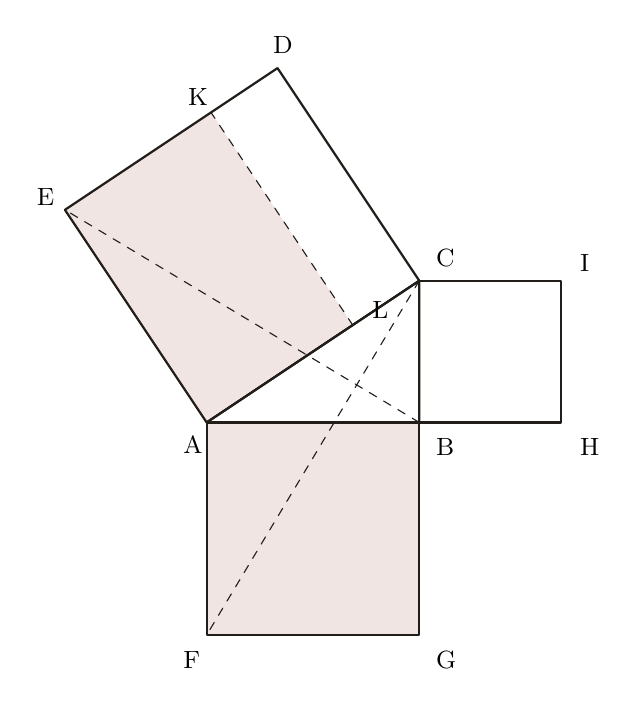
\begin{tikzpicture}[line cap=round,line join=round]
  \draw[fill=msred,fill opacity=0.13,draw=none] (1.80,4.14) -- (3.66,5.37) -- (1.86,8.07) -- (0.00,6.84) -- cycle;
  \draw[fill=msred,fill opacity=0.13,draw=none] (1.80,4.14) -- (4.50,4.14) -- (4.50,1.44) -- (1.80,1.44) -- cycle;
  \draw[msink,thick] (1.80,4.14) -- (4.50,5.94) -- (2.70,8.64) -- (0.00,6.84) -- cycle;
  \draw[msink,thick] (1.80,4.14) -- (4.50,4.14) -- (4.50,1.44) -- (1.80,1.44) -- cycle;
  \draw[msink,thick] (4.50,4.14) -- (4.50,5.94) -- (6.30,5.94) -- (6.30,4.14) -- cycle;
  \draw[msink,thick] (1.80,4.14) -- (4.50,4.14) -- (4.50,5.94) -- cycle;
  \draw[msink,dashed] (3.66,5.37) -- (1.86,8.07);
  \draw[msink,dashed] (4.50,4.14) -- (0.00,6.84);
  \draw[msink,dashed] (4.50,5.94) -- (1.80,1.44);
  % arc in the source figure, omitted: M 138 150 L 138 138 L 150 138
  \node[anchor=base west] at (1.38,3.75) {\small A};
  \node[anchor=base west] at (4.59,3.72) {\small B};
  \node[anchor=base west] at (4.59,6.12) {\small C};
  \node[anchor=base west] at (2.52,8.82) {\small D};
  \node[anchor=base west] at (-0.48,6.90) {\small E};
  \node[anchor=base west] at (1.44,8.16) {\small K};
  \node[anchor=base west] at (3.78,5.46) {\small L};
  \node[anchor=base west] at (1.38,1.02) {\small F};
  \node[anchor=base west] at (4.59,1.02) {\small G};
  \node[anchor=base west] at (6.42,3.72) {\small H};
  \node[anchor=base west] at (6.42,6.06) {\small I};
\end{tikzpicture}
\mscaption{Redrawn after the marginal figure. LK divides the square on AC into the two rectangles ALKE and LCDK; BE and CF are the joining lines.\footnote{The square on the hypotenuse is lettered A, C, D, E in the manuscript, with K the point in which the line from L meets the side ED; the two rectangles are then ALKE and LCDK, as the working has them. The joining lines BE and CF are drawn in the finest dotted line in the original.}}
\end{msfigure}

\dutchtext{Om te bewijsen, dat in een regthoekige driehoek ABC het quadraat op de hijpothoneuse AC\footnote{\textit{Hijpothoneuse} --- the spelling is the examiner's. \textit{De regte hoek zijde}, the sides about the right angle, Euclid's ``sides containing the right angle''.} Even zoo groot als de twee quadraten op de regte hoek zijde AB en BC te zamen Genoomen is.}
\engtext{To prove that in a right-angled triangle ABC the square on the hypotenuse AC is just as great as the two squares on the sides about the right angle, AB and BC, taken together.}

\worktitle{Bewijs}{Proof}
\begin{workblock}
  \wrow{}{$\angle EAC = \angle FAB$}{Both right, being angles of the two squares.}
  \wrow{addeert}{$\angle BAC = \angle BAC$}{The angle of the triangle, common to both.}\ruleunder
  \wrow{komt}{$\angle BAE = \angle FAC$}{The two included angles.}
  \wrow{}{$AE = AC$}{Two sides of the square on the hypotenuse.}
  \wrow{en}{$AB = AF$}{Two sides of the square on AB.}\ruleunder
  \wrow{derhalve}{$\triangle ABE = \triangle FAC$}{Two sides and the included angle.}
  \wrow{}{$2\,\triangle BAE = 2\,\triangle FAC$}{Each triangle is half of a figure on the same base and height.\footnote{The manuscript writes a stray ``/2'' at the end of the sixth line, where the doubling is being set up. The step is Euclid I.41: a parallelogram is double a triangle on the same base and between the same parallels --- the thirteenth example's theorem in another dress.}}\ruleunder
  \wrow{dat is}{$\square ALKE = \square ABFG$}{The first rectangle equals the square on AB.}
  \wnote{op de zelfde wijsen word ook beweese dat}
  \wrow{}{$\square LCDK = \square BCIH$}{And the second the square on BC.}\ruleunder
  \wnote{als men nu tot het $\square$ALKE = $\square$ABFG addeert $\square$LCDK = $\square$BCIH}
  \wrow{komt}{$AC^2 = AB^2 + BC^2$}{The two rectangles make the whole square on AC.}
  \wnote{'t welk te bewijse was.}
\end{workblock}

\reading{Euclid, \textit{Elements} I.47, by Euclid's own proof --- the windmill. The perpendicular from B cuts the square on the hypotenuse into two rectangles; each is shown equal to one of the squares on the legs, by way of a pair of triangles that is half of each. The examiner proves the first case in full and writes \textit{op de zelfde wijsen} --- ``in the same manner'' --- for the second, which is what every schoolbook does. It is worth noting that the paper has already used this theorem four times, in the seventh, eighth and ninth examples, before demonstrating it here; the examination is ordered by topic, not by dependence.}

\begin{msnotes}
  \item[4.] The machine transcription of this proof renders the angle glyph as L or I throughout --- \texttt{LEAC-ITAD} for $\angle$EAC = $\angle$FAB --- and the concluding line as \texttt{komt ac=a 4 p=a1 8co}. All readings taken from the scan.
\end{msnotes}

\clearpage
\parttitle{Lichamen en cirkels}{Solids and circles}{Examples 16--18 \textperiodcentered\ fol. 3604}

\foliomark{3604}{0037}{16--18}

\foliostand{Archimedes on the sphere \textperiodcentered{} the circle \textperiodcentered{} the mean proportional}{The last proofs on the paper; from the nineteenth example on, the examination calculates.}

\exempel{16de Exempel}{Sixteenth Example}

\begin{msfigure}
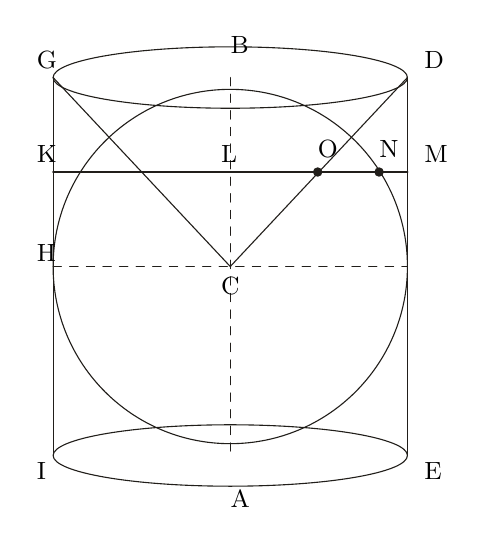
\begin{tikzpicture}[line cap=round,line join=round]
  \draw[msink] (3.60,5.70) ellipse (2.25 and 0.39);
  \draw[msink] (3.60,0.90) ellipse (2.25 and 0.39);
  \draw[msink] (1.35,5.70) -- (1.35,0.90);
  \draw[msink] (5.85,5.70) -- (5.85,0.90);
  \draw[msink] (3.60,3.30) circle (2.25);
  \draw[msink] (3.60,3.30) -- (1.35,5.70);
  \draw[msink] (3.60,3.30) -- (5.85,5.70);
  \draw[msink,dashed] (3.60,5.70) -- (3.60,0.90);
  \draw[msink,dashed] (1.35,3.30) -- (5.85,3.30);
  \draw[msink,thick] (1.35,4.50) -- (5.85,4.50);
  \fill[msink] (4.71,4.50) circle (0.06);
  \fill[msink] (5.49,4.50) circle (0.06);
  \node[anchor=base west] at (1.02,5.82) {\small G};
  \node[anchor=base west] at (3.48,6.00) {\small B};
  \node[anchor=base west] at (5.94,5.82) {\small D};
  \node[anchor=base west] at (1.02,4.62) {\small K};
  \node[anchor=base west] at (3.36,4.62) {\small L};
  \node[anchor=base west] at (4.59,4.68) {\small O};
  \node[anchor=base west] at (5.37,4.68) {\small N};
  \node[anchor=base west] at (5.94,4.62) {\small M};
  \node[anchor=base west] at (1.02,3.36) {\small H};
  \node[anchor=base west] at (3.36,2.94) {\small C};
  \node[anchor=base west] at (1.02,0.60) {\small I};
  \node[anchor=base west] at (3.48,0.24) {\small A};
  \node[anchor=base west] at (5.94,0.60) {\small E};
\end{tikzpicture}
\mscaption{Redrawn after the marginal figure: the cylinder GDEI, the sphere inscribed in it, and the cone standing on the top circle with its point at the centre C. KM is one cutting plane.\footnote{The manuscript draws the solid in a single small figure: the cylinder in outline with its two ellipses, the sphere inscribed, the cone as two straight lines from the centre C to the rim of the top circle, and the cutting plane as a line from K to M carrying the points O on the cone and N on the sphere. The cone stands point-downward, its apex at the centre of the sphere.}}
\end{msfigure}

\dutchtext{Om te Bewijsen, dat een kloot (Sphaera) twee derde deele van een Cylinder is, die met hem Een Gelijke grondvlakte en hoogte heeft.}
\engtext{To prove that a sphere is two-thirds of a cylinder having the same base and the same height as itself.}

\worktitle{Bewijs}{Proof}
\begin{workblock}
  \wrow{}{$CN^2 = CL^2 + LN^2$}{Pythagoras: N lies on the sphere, C is its centre.}
  \wrow{}{$CN^2 = LM^2$}{The radius of the sphere is the radius of the cylinder.}\ruleunder
  \wrow{dan is}{$LM^2 = CL^2 + LN^2$}{Substituting.}
  \wrow{}{$CL^2 = LO^2$}{The cone's side falls at half a right angle, so LO is CL.\footnote{Because the cylinder's height is its diameter, the cone from the centre to the top circle has its side at 45 degrees, so that LO --- the radius of its section --- always equals CL, the height above the centre. The examiner states the equality without the reason.}}\ruleunder
  \wrow{komt}{$LM^2 = LO^2 + LN^2$}{And squares on radii stand as the circles upon them.}
  \wnote{Dat is, het vlak der snijdinge der cijlinders is gelijk het vlak der snijdinge des keegels en der halve kloot te zame genoome; bij gevolg als de keegel $\tfrac13$ van de cijlinder is, zoo moet de kloot $\tfrac23$ van de zelve zijn.}
  \wnote{That is, the section of the cylinder is equal to the section of the cone and of the half sphere taken together; consequently, as the cone is one third of the cylinder, so must the sphere be two thirds of it.}
\end{workblock}

\reading{Archimedes' theorem, and the finest thing on the paper. Cut cylinder, sphere and cone by any plane parallel to the base: the circle of the cylinder is always equal to the circle of the cone and the circle of the sphere together, because their radii satisfy Pythagoras. Since this holds at every height, it holds of the solids --- and the cone being a third of the cylinder, the half sphere is a sixth short of a half, that is, the whole sphere is two thirds. The argument by cross-sections is Cavalieri's, from the seventeenth century, not Archimedes' own; it had become the schoolbook proof by 1787. It is also the theorem behind the twenty-third example's ratio of 300 to 157, which is nothing but two thirds of the cylinder written as a fraction of the cube.}

\begin{msnotes}
  \item[3.] \textit{Vlak der snijdinge} --- the plane of the cut, the cross-section; \textit{grondvlakte}, the base. The plural \textit{der cijlinders} is the hand's, for the singular.
  \item[4.] The step from ``every section is equal'' to ``the solids are equal'' is the whole content of the theorem and is passed over in the words \textit{bij gevolg}, ``consequently''. That the cone is a third of its cylinder is likewise assumed.
\end{msnotes}

\exempel{17de Exempel}{Seventeenth Example}

\begin{msfigure}
\begin{tikzpicture}[line cap=round,line join=round]
  \draw[msink,thick] (3.60,3.30) circle (2.55);
  \draw[msink,thick] (1.35,4.50) -- (5.85,4.50);
  \draw[msink] (3.60,5.85) -- (3.60,0.75);
  \draw[msink] (3.60,0.75) -- (1.35,4.50);
  \draw[msink] (3.60,0.75) -- (5.85,4.50);
  % arc in the source figure, omitted: M 120 25 A 85 85 0 0 0 45 70
  \fill[msink] (3.60,3.30) circle (0.07);
  \node[anchor=base west] at (3.45,6.06) {\small D};
  \node[anchor=base west] at (3.45,0.24) {\small E};
  \node[anchor=base west] at (0.96,4.38) {\small B};
  \node[anchor=base west] at (6.00,4.38) {\small A};
  \node[anchor=base west] at (3.42,4.74) {\small G};
  \node[anchor=base west] at (3.78,3.15) {\small O};
  \node[anchor=base west] at (1.56,4.08) {\small ℓ};
  \node[anchor=base west] at (5.52,4.08) {\small k};
  \node[anchor=base west] at (3.18,4.02) {\small m};
  \node[anchor=base west] at (3.84,4.02) {\small n};
  \node[anchor=base west] at (3.12,1.14) {\small h};
  \node[anchor=base west] at (3.90,1.14) {\small i};
\end{tikzpicture}
\mscaption{Redrawn after the marginal figure. DE cuts the chord AB at right angles in G; the arc BD is picked out.}
\end{msfigure}

\dutchtext{Om te bewijsen, dat wanneer de perpendiculaare lijn DE de coort AB\footnote{\textit{Coort} (modern \textit{koorde}) --- the chord, as \textit{pees} is in the twenty-first example; the two words are used interchangeably in the period, \textit{pees} keeping the bowstring metaphor and \textit{coort} being simply a cord.} bij G in twee Gelijke deele deelt, dezelve door het middelpunt O gaadt, en ook de Boog BEA in twee gelijke deele deelt.}
\engtext{To prove that when the perpendicular line DE divides the chord AB into two equal parts at G, the same passes through the centre O, and also divides the arc BEA into two equal parts.}

\worktitle{Bewijs}{Proof}
\begin{workblock}
  \wrow{}{$BG = GA$}{Given: the chord is bisected.}
  \wrow{}{$EG = EG$}{The common side.}
  \wrow{}{$\angle m = \angle n$}{Given: both right.}\ruleunder
  \wrow{dan is}{$\triangle BGE = \triangle AGE$}{Two sides and the included angle.}
  \wrow{daarom is}{$\angle h = \angle i$}{The angles at E.}
  \wrow{en}{$\angle \ell = \angle k$}{The angles at B and at A.}
  \wnote{
 \textit{Corol.\footnote{The two lines of the corollary are set in the manuscript within a large brace, with ditto marks carrying the words down from the first line to the second --- the only brace of its kind on the paper apart from the twelfth example's. The layout is reproduced here.}}
 
 Om dat de $\angle$h = $\angle$i is, zoo is de Boog BD = DA\\
 ''    ''   $\angle$ℓ = $\angle$k ; ''   ''   BE = EA
 
 }
  \wrow{komt de Boog}{$DBE = DAE$}{The two halves of the whole circumference.}
  \wnote{dan is ED de middellijn, gaande door 't middelpunt O, dat te bewijse was.}
\end{workblock}

\reading{Euclid, \textit{Elements} III.1 and III.3 taken together. The congruence of the two triangles gives equal angles at E and equal angles at the ends of the chord; equal inscribed angles stand on equal arcs, so the arcs BD and DA are equal and so are BE and EA; adding, the arc DBE equals the arc DAE, which is to say that DE divides the circle in half, and a line dividing a circle in half is a diameter. The examiner reaches the centre by way of the circumference --- the reverse of the usual route, and rather elegant.}

\begin{msnotes}
  \item[3.] The angles are lettered h and i at E, ℓ and k at the two ends of the chord, m and n at the foot G. The hand distinguishes ℓ from the angle glyph only by size; the machine transcription reads the whole family as L, I and 1 indifferently.
\end{msnotes}

\exempel{18de Exempel}{Eighteenth Example}

\begin{msfigure}
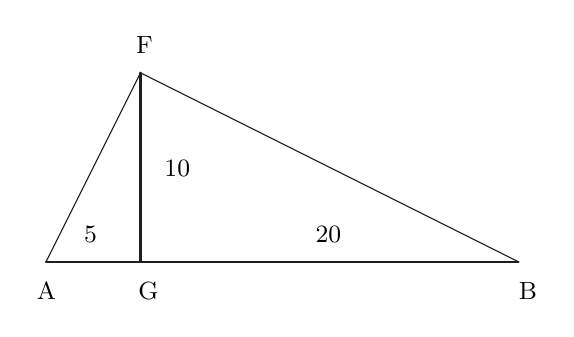
\begin{tikzpicture}[line cap=round,line join=round]
  % arc in the source figure, omitted: M 30 160 A 100 100 0 0 1 230 160
  \draw[msink,thick] (0.90,0.90) -- (6.90,0.90);
  \draw[msink] (0.90,0.90) -- (2.10,3.30);
  \draw[msink] (2.10,3.30) -- (6.90,0.90);
  \draw[msink,thick] (2.10,0.90) -- (2.10,3.30);
  \draw[msink] (2.10,0.90) -- (2.10,3.30);
  % arc in the source figure, omitted: M 70 148 L 82 148 L 82 160
  \node[anchor=base west] at (0.66,0.42) {\small A};
  \node[anchor=base west] at (1.95,0.42) {\small G};
  \node[anchor=base west] at (6.78,0.42) {\small B};
  \node[anchor=base west] at (1.92,3.54) {\small F};
  \node[anchor=base west] at (1.26,1.14) {\small 5};
  \node[anchor=base west] at (4.20,1.14) {\small 20};
  \node[anchor=base west] at (2.28,1.98) {\small 10};
\end{tikzpicture}
\mscaption{Redrawn after the marginal figure, with the examiner's own numbers written in as he wrote them.}
\end{msfigure}

\dutchtext{Om tusschen twee gegeevene Lijnen AG en GB een middel Evenreedige te vinden,\footnote{\textit{Middel evenreedige} --- the mean proportional, the geometric mean; the manuscript writes it both as two words and, in the answer, as one, \textit{Middelevenreedige}. \textit{Evenredig} is the ordinary Dutch for ``proportional''.} als meede met des zelvige Bewijs. Bij voorbeeld: laat zijn AG 5 en BG 20 voet. \textcolor{msred}{Antwoord, GF = 10 = de Middelevenreedige.}}
\engtext{To find a mean proportional between two given lines AG and GB, together with the proof of the same. For example, let AG be 5 and BG 20 feet. \textit{Answer: GF = 10, the mean proportional.}}

\worktitle{Bewijs}{Proof}
\begin{workblock}
  \wrow{
 
 
 
 
 
 \textit{dan is}
 
 
 }{$AG : GF = GF : GB$}{}
  \wrow{dat is}{$5 \times 20 = 100 \quad \textit{en}\quad GF = 10$}{}
  \wnote{dat te bewijse was.}
\end{workblock}

\reading{Euclid, \textit{Elements} VI.13 --- set the two lines end to end, describe a semicircle upon the whole, and the perpendicular at the joint is the mean proportional. It is the same rule the twenty-first example will use to find a diameter from a chord and its versine, here stated as a construction and verified on numbers. The example is a hinge: it is the last thing on the paper that carries a proof, and the first that ends in an arithmetical answer. Everything after it is calculation.}

\begin{msnotes}
  \item[2.] The reason is set in the manuscript to the right of the two lines of working, within a single large brace embracing both --- a layout the hand reserves for a justification that governs more than one line. It is reproduced here as a rule with the reason alongside.
  \item[3.] \textit{Gelijkformig} --- similar, of figures alike in shape but not in size; the modern Dutch is \textit{gelijkvormig}. That the angle at F is right, which is what makes the two triangles similar, is not stated; it is the twenty-first example's angle in a semicircle.
  \item[4.] The heading of the nineteenth example stands at the foot of this page, the example itself beginning on the next opening.
\end{msnotes}

\clearpage
\parttitle{Meetkonst}{Mensuration by the rule of three}{Examples 19--30 \textperiodcentered\ fol. 3605--3607}

\foliomark{3605}{0038}{19--23}

\foliostand{The circle and the sphere \textperiodcentered{} mensuration by rule of three}{}

\exempel{19de Exempel}{Nineteenth Example}

\begin{msfigure}
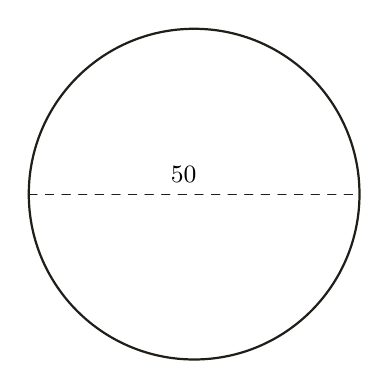
\begin{tikzpicture}[line cap=round,line join=round]
  \draw[msink,thick] (3.60,2.55) circle (2.10);
  \draw[msink,dashed] (1.50,2.55) -- (5.70,2.55);
  \node[anchor=base west] at (3.18,2.70) {\small 50};
\end{tikzpicture}
\mscaption{The scribe's sketch: a circle with 50 written along the diameter --- the answer, not the datum.}
\end{msfigure}

\dutchtext{Om uijt de gegeevene Inhoud van een Rond, de Middelijn te vinden.\footnote{\textit{Rond} --- a circle, as a plane figure; \textit{middelijn} (modern \textit{middellijn}) the diameter; \textit{inhoud} the content, here the area, and in the later examples the volume. \textit{Voet}, the Rijnland foot of 0\textperiodcentered{}3139 m; the answers are in feet and square feet as the school reckoned them, not in any surveyed measure.} Bij voorbeelt: Laat den Inhoud 1962$\tfrac12$ quadraat voeten\footnote{1962$\tfrac12$ is exact for the ratio used: 2500 $\times$ 0\textperiodcentered{}785 = 1962\textperiodcentered{}5. The true area of a circle of diameter 50 is 1963\textperiodcentered{}50 square feet, so the school ratio runs about one part in two thousand light --- immaterial at the scale of a ship's reckoning.} zijn; hoe groot is de Middelijn? \textcolor{msred}{Antwoord 50 voeten.}}
\engtext{To find the diameter of a circle from its given area. For example: let the area be 1962$\tfrac12$ square feet; how great is the diameter? \textit{Answer: 50 feet.}}

\worktitle{Bewerking}{Working}
\begin{workblock}
  \wprop{\mscirc{} inhoud : $\square$ op de Middelijn \msprop{} \mscirc{} inhoud : $\square$ op de Middelijn}{$785 : 1000 = 1962\tfrac{1}{2} : 2500$}{}
\end{workblock}

\reading{Inverting the usual rule. The circle stands to the square on its diameter as 785 to 1000;\footnote{785 : 1000 is $\pi$/4 to three places (0\textperiodcentered{}7854). The symbol \mscirc{} for a circle and $\square$ for the square on a line are the manuscript's own; the four-term proportion is written with a colon for ratio and a long equals for the proportion itself, the eighteenth-century Dutch convention where later notation uses \msprop{}.} given the circle, the fourth proportional yields the square on the diameter, and the square root yields the diameter itself.\footnote{The manuscript writes the extraction in the long-division frame, \texttt{2|5|00|50}, with the digits of the root set to the right of the bar. It is rendered here as a radical for legibility; the working itself is not transcribed, being a scratch calculation rather than a statement.} The examiner does not write $\pi$ and does not need it: the whole of circle mensuration on this page is carried by three memorised integer ratios --- 785 : 1000 for area to square, 100 : 314 for diameter to circumference, 300 : 157 for cube to sphere.}

\exempel{20ste Exempel}{Twentieth Example}

\begin{msfigure}
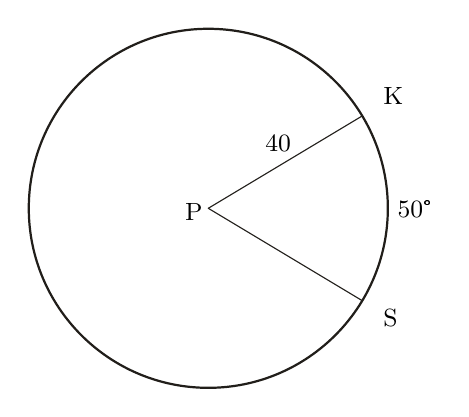
\begin{tikzpicture}[line cap=round,line join=round]
  % arc in the source figure, omitted: M 110 90 L 175 51 A 76 76 0 0 1 175 129 Z
  \draw[msink,thick] (3.30,2.70) circle (2.28);
  \draw[msink] (3.30,2.70) -- (5.25,3.87);
  \draw[msink] (3.30,2.70) -- (5.25,1.53);
  \node[anchor=base west] at (2.88,2.55) {\small P};
  \node[anchor=base west] at (5.40,4.02) {\small K};
  \node[anchor=base west] at (5.40,1.20) {\small S};
  \node[anchor=base west] at (3.90,3.42) {\small 40};
  \node[anchor=base west] at (5.58,2.58) {\small 50\textdegree{}};
\end{tikzpicture}
\mscaption{Redrawn after the marginal sketch: radius PK = 40 feet, arc KS = 50 degrees, the sector shaded.}
\end{msfigure}

\dutchtext{Als de Radius off Straal van een rond, KP, is 40 voete, en de groote van de Boog KS 50 gr. gegeeven is, om den inhoud van den Sector off Sneede\footnote{\textit{Sneede}, a cut or slice, glosses the Latin \textit{sector} for a reader who might not have it; the manuscript pairs Dutch and learned terms in this way throughout (\textit{kloot / Sphaera} in the two examples following).} KSP van het zelve rond te vinden. \textcolor{msred}{Antwoord 697 \vfrac{7}{9} quadraat voeten.}}
\engtext{Given that the radius or semidiameter of a circle, KP, is 40 feet, and the arc KS is 50 degrees, to find the area of the sector or slice KSP of that same circle. \textit{Answer: 697 \vfrac{7}{9} square feet.}}

\worktitle{Bewerking}{Working}
\begin{workblock}
  \wprop{Middelijn : omtrek \msprop{} $\tfrac12$ middelijn : $\tfrac12$ omtrek}{$100 : 314 = 40 : 125\tfrac{3}{5}$}{$\tfrac12$ omtrek in gr. : $\tfrac12$ omtrek in lijne \msprop{} KS in gr. : KS in lijne}
\end{workblock}

\reading{Three steps, each a rule of three. The radius gives the half-circumference;\footnote{The proportion is stated for diameter to circumference but applied to their halves, which is why 40 --- the radius --- yields 125 \vfrac{3}{5}, the \textit{half} circumference. 100 : 314 is $\pi$ to two places. The manuscript's \textit{Middel\textsuperscript{n}} is the ordinary abbreviation for \textit{middelijn}.} the half-circumference, being 180 degrees, gives the arc of 50 degrees in feet; and the arc multiplied by half the radius gives the sector. The examiner writes that multiplier as ``$\tfrac14$ van de Middelijn'' rather than ``$\tfrac12$ van de Straal'',\footnote{The rule is that a sector equals half its arc times the radius. The manuscript performs it as \textit{Multipl.} of 34 \vfrac{8}{9} by 20, the 20 glossed as a quarter of the diameter of 80 --- that is, half the radius --- so that the arc is taken whole and the radius halved rather than the reverse.} which is the same quantity and the more natural expression when the diameter is the school's standard of reference. The result, 697 \vfrac{7}{9}, is exact for the ratios used.\footnote{Checked against modern values: a 50\textdegree{} sector of radius 40 measures 698\textperiodcentered{}13 square feet. The school ratios give 697\textperiodcentered{}78 --- an error of one part in two thousand, inherited from 314 / 100.}}

\exempel{21ste Exempel}{Twenty-first Example}

\begin{msfigure}
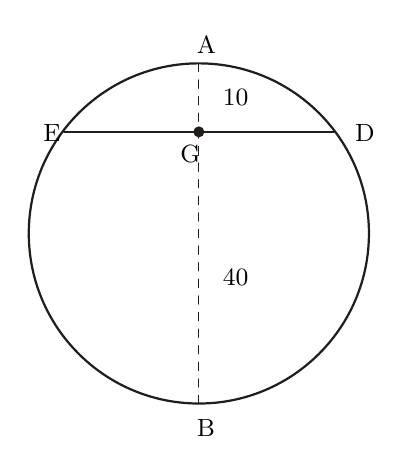
\begin{tikzpicture}[line cap=round,line join=round]
  \draw[msink,thick] (3.60,2.70) circle (2.16);
  \draw[msink,dashed] (3.60,4.86) -- (3.60,0.54);
  \draw[msink,thick] (1.89,3.99) -- (5.31,3.99);
  \fill[msink] (3.60,3.99) circle (0.07);
  \node[anchor=base west] at (3.45,4.98) {\small A};
  \node[anchor=base west] at (3.45,0.12) {\small B};
  \node[anchor=base west] at (1.50,3.87) {\small E};
  \node[anchor=base west] at (5.46,3.87) {\small D};
  \node[anchor=base west] at (3.24,3.60) {\small G};
  \node[anchor=base west] at (3.78,4.32) {\small 10};
  \node[anchor=base west] at (3.78,2.04) {\small 40};
\end{tikzpicture}
\mscaption{Redrawn after the marginal sketch: chord ED = 40, versine AG = 10, GB found as 40.}
\end{msfigure}

\dutchtext{Om uijt een gegeevene pees van een boog ED, en de pijl van de zelve AG, de middelijn AB te vinden.\footnote{\textit{Pees} --- literally a bowstring --- is the chord of an arc; \textit{pijl} --- the arrow --- is the versine, the perpendicular from the middle of the chord to the arc. The pair is the standard Dutch idiom, and the metaphor of the drawn bow is exactly the figure: string, arrow, and the bow itself.} Bij voorbeelt: laat zijn de pees ED 40 voete zijn, en de pijl AG 10 voete; hoe groot is de Middelijn? \textcolor{msred}{Antwoord 50 voeten.}}
\engtext{To find the diameter AB from a given chord of an arc, ED, and the versine of the same, AG. For example: let the chord ED be 40 feet and the versine AG 10 feet; how great is the diameter? \textit{Answer: 50 feet.}}

\worktitle{Bewerking}{Working}
\begin{workblock}
  \wrow{}{$AG : GD = GD : GB$}{}
\end{workblock}

\reading{The half-chord GD is a mean proportional\footnote{Written as a continued proportion with GD in both middle places, the eighteenth-century way of stating a mean proportional. It holds because the angle in a semicircle is right (Euclid III.31), so ED and AB are two chords cutting at G and AG $\times$ GB = GD $\times$ GE = GD$^{2}$.} between the two segments AG and GB of the diameter it stands on --- Euclid VI.13, or in the form the schools taught it, the rule that the rectangle on the segments of one chord equals that on the segments of the other. Given AG = 10 and GD = 20, GB is 40; add back the versine\footnote{\textit{Adeert} (modern \textit{addeert}), from Latin \textit{addere}, stands in the operator column exactly as \textit{substraheert} and \textit{trekt … aff} do elsewhere in the examination; the four school operations are named in the same hand throughout.} and the diameter is 50. This is the practical problem of the arc: a shipwright or a surveyor measures the chord and the rise, and wants the circle they belong to. Note that no square root is needed here, unlike the nineteenth example --- the mean-proportional form does the work.\footnote{The figures are chosen so that everything falls out whole, as is usual in these papers: 10, 20, 40, 50. The examiner tests the rule, not the arithmetic.}}

\exempel{22ste Exempel}{Twenty-second Example}

\begin{msfigure}
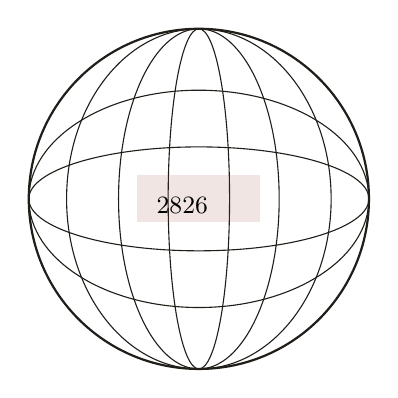
\begin{tikzpicture}[line cap=round,line join=round]
  \draw[msink,thick] (3.60,2.70) circle (2.16);
  \draw[msink] (3.60,2.70) ellipse (1.68 and 2.16);
  \draw[msink] (3.60,2.70) ellipse (1.02 and 2.16);
  \draw[msink] (3.60,2.70) ellipse (0.39 and 2.16);
  \draw[msink] (3.60,2.70) ellipse (2.16 and 1.38);
  \draw[msink] (3.60,2.70) ellipse (2.16 and 0.66);
  \draw[fill=msred,fill opacity=0.13,draw=none] (2.82,2.40) rectangle (4.38,3.00);
  \node[anchor=base west] at (2.94,2.52) {\small 2826};
\end{tikzpicture}
\mscaption{The scribe draws the sphere as a hatched ball, the datum written across it.\footnote{\textit{Kloot} is the ordinary Dutch word for a ball or globe, used of the terrestrial sphere as well; the manuscript glosses it \textit{(Sphaera)} in parentheses on first use, and again in the next example. The hatched ball is the scribe's conventional way of showing a solid rather than a plane figure.}}
\end{msfigure}

\dutchtext{Als de oppervlakte\footnote{\textit{Oppervlakte}, surface, is carefully distinguished from \textit{inhoud}, content --- which in the next example means volume. The manuscript's abbreviation \textit{oppervl.} and the superscript \textit{d\textsuperscript{e}} forms are expanded silently here.} van een kloot (Sphaera) is 2826 quadraat voete, hoe groot is dan de Middelijn? \textcolor{msred}{Antwoord 30 voeten.}}
\engtext{If the surface of a sphere is 2826 square feet, how great then is the diameter? \textit{Answer: 30 feet.}}

\worktitle{Bewerking}{Working}
\begin{workblock}
  \wprop{oppervl. : inhoud van de groote \mscirc{} \msprop{} oppervl. : inhoud}{$4 : 1 = 2826 : 706\tfrac{1}{2}$}{\mscirc{} inhoud : $\square$ Middelijn \msprop{} \mscirc{} inhoud : $\square$ Middelijn}
\end{workblock}

\reading{Two proportions and a root, chained: Archimedes' theorem that the surface of a sphere is four times its greatest circle\footnote{The ratio 4 : 1 is Archimedes, \textit{On the Sphere and Cylinder} I.33, transmitted to the reckoning schools as a bare rule without attribution. \textit{Groote \mscirc{}} --- the great circle, the section through the centre.} reduces the problem to the nineteenth example, which is then run backwards a second time. The examiner does not restate that earlier rule but writes it out in full again --- the examination rewards the visible working, not the economy of it. All the numbers are exact for the ratios used: 2826 / 4 = 706$\tfrac12$, and 706$\tfrac12$ / 0\textperiodcentered{}785 = 900.\footnote{True surface for a diameter of 30 is 2827\textperiodcentered{}43 square feet; the paper's 2826 is the figure the school ratios produce, and the question is set from the answer backwards so that it comes out whole.}}

\exempel{23ste Exempel}{Twenty-third Example}

\begin{msfigure}
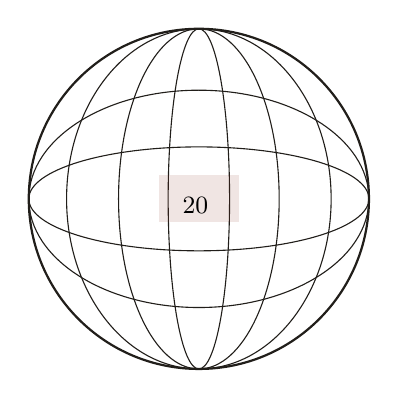
\begin{tikzpicture}[line cap=round,line join=round]
  \draw[msink,thick] (3.60,2.70) circle (2.16);
  \draw[msink] (3.60,2.70) ellipse (1.68 and 2.16);
  \draw[msink] (3.60,2.70) ellipse (1.02 and 2.16);
  \draw[msink] (3.60,2.70) ellipse (0.39 and 2.16);
  \draw[msink] (3.60,2.70) ellipse (2.16 and 1.38);
  \draw[msink] (3.60,2.70) ellipse (2.16 and 0.66);
  \draw[fill=msred,fill opacity=0.13,draw=none] (3.09,2.40) rectangle (4.11,3.00);
  \node[anchor=base west] at (3.27,2.52) {\small 20};
\end{tikzpicture}
\mscaption{The companion figure to the preceding example, the diameter written across it.}
\end{msfigure}

\dutchtext{Als de Middelijn van een kloot (Sphaera) is 20 voete, hoe groot is de Inhoud? \textcolor{msred}{Antwoord 4186 \vfrac{2}{3} cubicq\footnote{\textit{Cubicq} (Latin \textit{cubicus}) both as the cube of a number and as the cubic foot of the answer; the same word does the arithmetical and the metrological work, as \textit{quadraat} does for squares and square feet.} voete.}}
\engtext{If the diameter of a sphere is 20 feet, how great is the volume? \textit{Answer: 4186 \vfrac{2}{3} cubic feet.}}

\worktitle{Bewerking}{Working}
\begin{workblock}
  \wprop{Cubicq op de Middelijn : inhoud \msprop{} Cubicq op de Middelijn : inhoud}{$300 : 157 = 8000 : 4186\tfrac{2}{3}$}{}
\end{workblock}

\reading{The shortest working on the page, and the last of the series: a single rule of three against the cube on the diameter. 20 cubed is 8000;\footnote{The machine transcription reads the operative line as \texttt{300 : 157 = 0000 : 4186 2/3}, losing the 8 of 8000; the manuscript is clear. Corrected against the scan.} 8000 $\times$ 157 / 300 is 4186 \vfrac{2}{3}.\footnote{157 / 300 = 0\textperiodcentered{}52333, against $\pi$ / 6 = 0\textperiodcentered{}523599 --- a ratio derived from the same 314 / 100 the page uses elsewhere. The rule descends from Archimedes' result that a sphere is two-thirds of its circumscribing cylinder.} The three ratios the examiner has used across these five examples --- 785 : 1000, 100 : 314, 300 : 157 --- are the same constant in three dresses, $\pi$ / 4, $\pi$ and $\pi$ / 6, memorised as integers because integer proportions could be worked on paper at sea by anyone who had learned the rule of three.\footnote{True volume for a diameter of 20 is 4188\textperiodcentered{}79 cubic feet; the paper's 4186 \vfrac{2}{3} is short by one part in two thousand, the constant signature of the 314 / 100 approximation across the whole examination.}}

\foliomark{3606}{0039}{24--27}

\foliostand{Solid measure \textperiodcentered{} cylinder, prism, truncated cone, pyramid}{Every answer here is a base multiplied by a height, or a third of one.}

\exempel{24ste Exempel}{Twenty-fourth Example}

\begin{msfigure}
\begin{tikzpicture}[line cap=round,line join=round]
  \draw[msink,thick] (2.70,5.25) ellipse (1.35 and 0.36);
  % arc in the source figure, omitted: M 45 35 L 45 175 A 45 12 0 0 0 135 175 L 135 35
  \draw[msink,dashed] (2.70,5.25) -- (2.70,1.05);
  \node[anchor=base west] at (0.66,2.94) {\small 50};
  \node[anchor=base west] at (2.40,0.54) {\small 40};
\end{tikzpicture}
\mscaption{The scribe's hatched cylinder, with 50 written beside it and 40 across the base.}
\end{msfigure}

\dutchtext{Hoe groot is de inhoud van een Cylinder, wiens middelijn van de grondvlakte is 40 voet, en zijn hoogte 50 voet? \textcolor{msred}{Antwoord 62800 cubic voet.}}
\engtext{How great is the content of a cylinder whose base diameter is 40 feet and whose height is 50 feet? \textit{Answer: 62,800 cubic feet.}}

\worktitle{Bewerking}{Working}
\begin{workblock}
  \wnote{Middelijn : omtrek \msprop{} mid. : omtrek}
  \wrow{}{$125\tfrac{3}{5}$}{}
\end{workblock}

\reading{The base is found not by squaring the radius but by multiplying the circumference by a quarter of the diameter --- the old surveyor's rule, and the same one the twentieth example used on the sector. It is the more convenient of the two when the circumference has already been computed, as here it has. From there the solid is base times height, and the paper does not pause to say so.}

\begin{msnotes}
  \item[1.] Circumference times a quarter of the diameter is 2$\pi$r $\times$ r/2 = $\pi$r$^{2}$, the area of the circle; the rule is exact, not an approximation, and only the value of 314 / 100 introduces any error. 125\textperiodcentered{}6 $\times$ 10 = 1256, and 1256 $\times$ 50 = 62,800, both exact for the ratio used.
  \item[2.] The manuscript writes the successive multiplicands one beneath the other with a rule between, as in a ledger; each rule marks a completed multiplication, not an equation. The layout is reproduced.
  \item[3.] True volume for these dimensions is 62,831\textperiodcentered{}85 cubic feet.
\end{msnotes}

\exempel{25ste Exempel}{Twenty-fifth Example}

\begin{msfigure}
\begin{tikzpicture}[line cap=round,line join=round]
  \draw[msink] (1.20,5.40) -- (4.20,5.40) -- (2.70,4.56) -- cycle;
  \draw[msink,dashed] (2.70,5.40) -- (2.70,4.56);
  % arc in the source figure, omitted: M 40 40 L 40 180 L 90 200 L 140 180 L 140 40
  \draw[msink,dashed] (2.70,4.56) -- (2.70,0.60);
  \node[anchor=base west] at (0.90,5.58) {\small D};
  \node[anchor=base west] at (4.08,5.58) {\small G};
  \node[anchor=base west] at (2.10,5.04) {\small E};
  \node[anchor=base west] at (2.82,4.74) {\small B};
  \node[anchor=base west] at (2.52,0.18) {\small A};
  \node[anchor=base west] at (1.80,4.86) {\small 10};
  \node[anchor=base west] at (2.94,2.70) {\small 30};
\end{tikzpicture}
\mscaption{Redrawn after the marginal figure: the prism stands on end, its triangular face uppermost.\footnote{The manuscript draws the prism upright and heavily hatched down its length, with the triangular face foreshortened at the top and the letters D, E, B, G crowded into it; A stands at the foot. The proportions here are the figure's, not the problem's.}}
\end{msfigure}

\dutchtext{Om gegeeve zijnde de zijde DB 18 voete, en de hoogte EG 10 voet, met de geheele hoogte van de prisma 30 voet; de inhoud van de zelve te vinden. \textcolor{msred}{Antwoord 2700 cubic voete} = de inhoud van de Prisma.}
\engtext{Given the side DB 18 feet and the height EG 10 feet, with the whole height of the prism 30 feet, to find the content of the same. \textit{Answer: 2700 cubic feet, the content of the prism.}}

\worktitle{Bewerking}{Working}
\begin{workblock}
  \wrow{}{$DB = 18$}{}
\end{workblock}

\reading{The triangle is taken as its base by half its height --- the examiner halves the 10 before multiplying rather than halving the product, which is what a reckoner does when the halving comes out whole. The prism is then that base by its length, exactly as the cylinder was. Placed side by side, the twenty-fourth and twenty-fifth examples make the same point twice over: for any solid of constant section, the content is the section times the height, whatever the shape of the section.}

\begin{msnotes}
  \item[2.] The base triangle is named DBC in the working but D, B and G in the proposition and the figure; the hand is inconsistent. 18 $\times$ 5 = 90 and 90 $\times$ 30 = 2700, both exact.
  \item[3.] \textit{Prisma} is used as a feminine noun --- \textit{de prisma}, \textit{van de Prisma} --- as are \textit{de pijramide} and \textit{de keegel} elsewhere on the paper.
\end{msnotes}

\exempel{26ste Exempel}{Twenty-sixth Example}

\begin{msfigure}
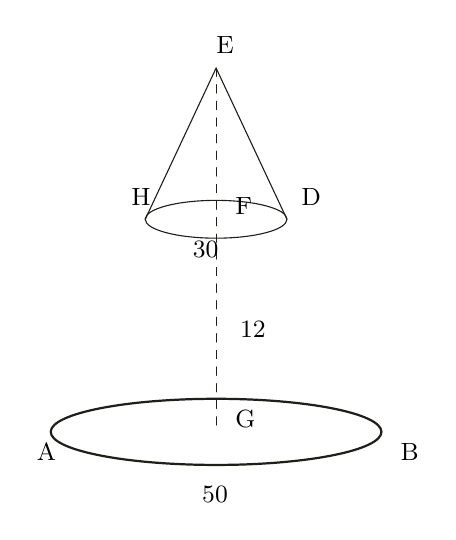
\begin{tikzpicture}[line cap=round,line join=round]
  \draw[msink] (2.10,3.90) -- (3.00,5.82);
  \draw[msink] (3.90,3.90) -- (3.00,5.82);
  \draw[msink] (3.00,3.90) ellipse (0.90 and 0.24);
  % arc in the source figure, omitted: M 30 180 L 70 90 M 170 180 L 130 90
  \draw[msink,thick] (3.00,1.20) ellipse (2.10 and 0.42);
  \draw[msink,dashed] (3.00,5.82) -- (3.00,1.20);
  % arc in the source figure, omitted: M 30 180 L 70 90 L 130 90 L 170 180 Z
  \node[anchor=base west] at (2.88,6.00) {\small E};
  \node[anchor=base west] at (1.80,4.08) {\small H};
  \node[anchor=base west] at (3.96,4.08) {\small D};
  \node[anchor=base west] at (3.12,3.96) {\small F};
  \node[anchor=base west] at (0.60,0.84) {\small A};
  \node[anchor=base west] at (5.22,0.84) {\small B};
  \node[anchor=base west] at (3.12,1.26) {\small G};
  \node[anchor=base west] at (2.58,3.42) {\small 30};
  \node[anchor=base west] at (3.18,2.40) {\small 12};
  \node[anchor=base west] at (2.70,0.30) {\small 50};
\end{tikzpicture}
\mscaption{Redrawn after the marginal figure. The small cone HED that completes the frustum is drawn in dotted line, as in the original.}
\end{msfigure}

\dutchtext{Hoe groot is de inhoud van een afgekorte keegel ABDH,\footnote{\textit{Afgekorte keegel}, and below \textit{gekorte keegel} and \textit{korte keegel} --- three forms for the frustum within one example, all meaning the shortened cone. The solid is lettered ABDH in the proposition and AHDB in the answer.} wiens middellijn van de grondvlakte AB is 50 voet en HD 30 voet, en de hoogte van de gekorte keegel FG 12 voet? \textcolor{msred}{Antwoord 15386 cubic voeten.}}
\engtext{How great is the content of a truncated cone ABDH whose base diameter AB is 50 feet and HD 30 feet, and the height of the truncated cone FG 12 feet? \textit{Answer: 15,386 cubic feet.}}

\worktitle{Bewerking}{Working}
\begin{workblock}
  \wnote{{\color{msmut}\small fol. 3606\textsuperscript{v}}}
  \wnote{First, the height of the whole cone\footnote{AG is half the difference of the two diameters, 10; GH is the height of the frustum, 12; AC is the base radius, 25; GE the height of the whole cone, 30. The first proportion is thus the similar triangles of the cone's profile, and the examiner writes it without comment at the head of the page.}}
  \wnote{Then the small cone HED}
  \wrow{}{$7\tfrac{1}{2}$}{}\ruleunder
  \wnote{Then the whole cone AEB}
  \wrow{}{$12\tfrac{1}{2}$}{}\ruleunder
\end{workblock}

\reading{The longest working on the paper, and the only one that runs to three separate calculations. The frustum is measured by completing it: find where the sides would meet by similar triangles, measure the whole cone, measure the small cone that has been cut off, and subtract. The difference of the radii, 10, is to the height of the frustum, 12, as the great radius, 25, is to the whole height, 30 --- and the small cone's height is therefore 18, of which a third is 6. Every figure comes out whole, and the answer, 15,386, is exact for the ratio 314 to 100.}

\begin{msnotes}
  \item[3.] The proposition stands at the foot of the recto with \textit{'t werk volgt}; the three calculations occupy the head of the verso. They are set here as one continuous working, with the manuscript's ditto marks kept in the final subtraction.
  \item[4.] True volume is 15,393\textperiodcentered{}8 cubic feet; the shortfall of about one part in two thousand is again the 314 / 100.
\end{msnotes}

\exempel{27ste Exempel}{Twenty-seventh Example}

\begin{msfigure}
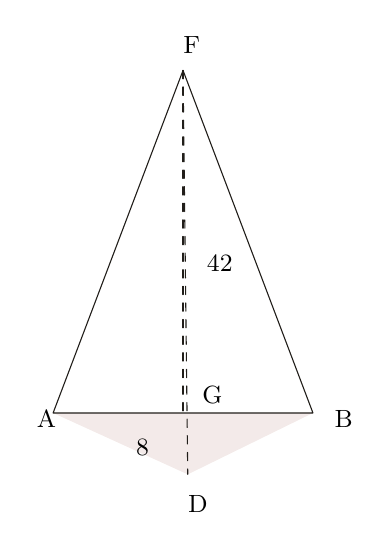
\begin{tikzpicture}[line cap=round,line join=round]
  \draw[fill=msred,fill opacity=0.10,draw=none] (1.05,1.50) -- (4.35,1.50) -- (2.76,0.72) -- cycle;
  \draw[msink] (2.70,5.85) -- (1.05,1.50) -- (4.35,1.50) -- cycle;
  % arc in the source figure, omitted: M 35 170 L 92 196 L 145 170
  \draw[msink,dashed] (2.70,5.85) -- (2.76,0.72);
  \draw[msink,dashed] (2.70,5.85) -- (2.70,1.50);
  \node[anchor=base west] at (2.58,6.06) {\small F};
  \node[anchor=base west] at (0.72,1.32) {\small A};
  \node[anchor=base west] at (4.50,1.32) {\small B};
  \node[anchor=base west] at (2.64,0.24) {\small D};
  \node[anchor=base west] at (2.82,1.62) {\small G};
  \node[anchor=base west] at (2.88,3.30) {\small 42};
  \node[anchor=base west] at (1.98,0.96) {\small 8};
\end{tikzpicture}
\mscaption{Redrawn after the marginal figure. AB is the base of the triangle ABD, BG its height; DF is the height of the pyramid.}
\end{msfigure}

\dutchtext{Om gegeeven zijnde AD 15 voet, en de hoogte BG 8 voet, met de geheele hoogte DF van de driekantige pijramide 42 voet,\footnote{The height is written 42 in the figure and, less legibly, in the proposition; the working confirms it, since a third of DF is given as 14. \textit{Driekantig}, three-sided, of a pyramid on a triangular base.} den inhoud van de zelve te vinden. \textcolor{msred}{Antwoord 840 cubic voete.}}
\engtext{Given AD 15 feet, and the height BG 8 feet, with the whole height DF of the three-sided pyramid 42 feet, to find the content of the same. \textit{Answer: 840 cubic feet.}}

\worktitle{Bewerking}{Working}
\begin{workblock}
  \wrow{}{$AD = 15$}{}
\end{workblock}

\reading{Base by a third of the height --- the rule for every pointed solid, and the same one the cones of the previous example used. The examiner halves the 8 first to get the triangle, then takes a third of the 42 before multiplying, so that both awkward divisions are done on small whole numbers and the multiplication is left clean. The last three lines are the long multiplication of 60 by 14 written out in the ordinary way, the 240 and the 60 being the partial products.}

\begin{msnotes}
  \item[2.] The partial products 240 and 60 stand for 60 $\times$ 4 and 60 $\times$ 10, the second shifted a place; the manuscript does not align them, writing both flush and relying on the reader to know the rule. 60 $\times$ 14 = 840, exact.
  \item[3.] This is the only answer on the paper with no approximation in it at all: no circle enters the calculation, so no value of $\pi$ is needed.
\end{msnotes}

\foliomark{3607}{0040}{28--30}

\foliostand{The last three \textperiodcentered{} pyramid, circumscribed circle, icosahedron}{The paper ends here; the leaf below the thirtieth example is left blank.}

\exempel{28ste Exempel}{Twenty-eighth Example}

\begin{msfigure}
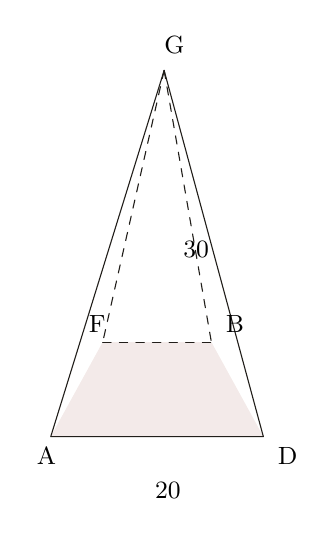
\begin{tikzpicture}[line cap=round,line join=round]
  \draw[fill=msred,fill opacity=0.10,draw=none] (1.20,1.20) -- (3.90,1.20) -- (3.24,2.40) -- (1.86,2.40) -- cycle;
  \draw[msink] (2.64,5.85) -- (1.20,1.20) -- (3.90,1.20) -- cycle;
  % arc in the source figure, omitted: M 40 180 L 62 140 L 108 140 L 130 180
  \draw[msink,dashed] (2.64,5.85) -- (1.86,2.40);
  \draw[msink,dashed] (2.64,5.85) -- (3.24,2.40);
  \draw[msink,dashed] (1.86,2.40) -- (3.24,2.40);
  \node[anchor=base west] at (2.52,6.06) {\small G};
  \node[anchor=base west] at (0.90,0.84) {\small A};
  \node[anchor=base west] at (3.96,0.84) {\small D};
  \node[anchor=base west] at (1.56,2.52) {\small F};
  \node[anchor=base west] at (3.30,2.52) {\small B};
  \node[anchor=base west] at (2.76,3.48) {\small 30};
  \node[anchor=base west] at (2.40,0.42) {\small 20};
\end{tikzpicture}
\mscaption{Redrawn after the marginal figure: the square base ADBF is drawn in perspective, the height DG running to the apex.}
\end{msfigure}

\dutchtext{Hoe groot is den inhoud van een gelijkzijdige vierkantige pijramied,\footnote{\textit{Gelijkzijdige vierkantige pijramied} --- ``equilateral four-cornered pyramid'', that is, one on a square base; \textit{vierkantig} refers to the base, \textit{gelijkzijdig} to its being regular. The base is lettered ADBF, its corners taken round the figure as the eye meets them.} wiens eene zijd van de grondvlakte AD is 20 voet, en zijn hoogte DG 30 voet? \textcolor{msred}{Antwoord 4000 cubiq voete.}}
\engtext{How great is the content of a regular square pyramid, one side of whose base AD is 20 feet and whose height DG is 30 feet? \textit{Answer: 4000 cubic feet.}}

\worktitle{Bewerking}{Working}
\begin{workblock}
  \wrow{}{$AD = 20$}{}
\end{workblock}

\reading{The same rule as the example before, on a square base instead of a triangular one, and with figures chosen so that the whole working is three multiplications of round numbers. Nothing is explained, because by this point in the paper nothing needs to be: the rule of base times a third of the height has been established, and the section is now simply demonstrating that it applies to whatever base is set before it.}

\begin{msnotes}
  \item[2.] The manuscript sets the second 20 with a small pair of quote-like marks to its left, its sign for ``the same again'' in a multiplication of a number by itself --- the same device as the 29th example's repeated OK and KN.
\end{msnotes}

\exempel{29ste Exempel}{Twenty-ninth Example}

\begin{msfigure}
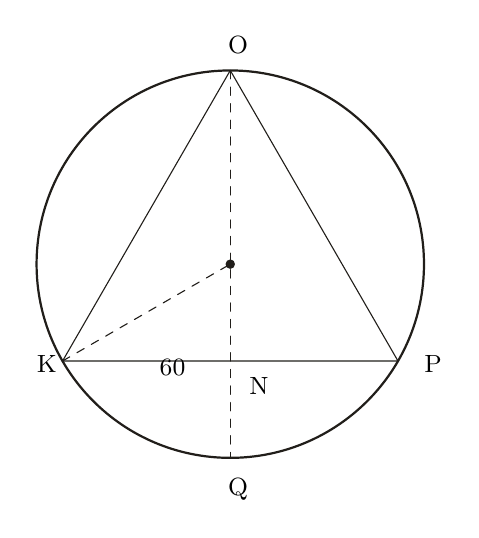
\begin{tikzpicture}[line cap=round,line join=round]
  \draw[msink,thick] (3.00,3.15) circle (2.46);
  \draw[msink] (3.00,5.61) -- (0.87,1.92) -- (5.13,1.92) -- cycle;
  \draw[msink,dashed] (3.00,5.61) -- (3.00,0.69);
  \draw[msink,dashed] (0.87,1.92) -- (3.00,3.15);
  \fill[msink] (3.00,3.15) circle (0.06);
  \node[anchor=base west] at (2.85,5.82) {\small O};
  \node[anchor=base west] at (0.42,1.77) {\small K};
  \node[anchor=base west] at (5.34,1.77) {\small P};
  \node[anchor=base west] at (2.85,0.21) {\small Q};
  \node[anchor=base west] at (3.12,1.50) {\small N};
  \node[anchor=base west] at (1.98,1.74) {\small 60};
\end{tikzpicture}
\mscaption{Redrawn after the marginal figure: the equilateral triangle KOP in its circle, with the diameter OQ cutting KP at N.}
\end{msfigure}

\dutchtext{Als de zijde KP van een gelijkzijdige driehoek KOP is 60 voet; hoe groot is dan de Radius van een circul die om de zelve driehoek kan beschreeven worden? \textcolor{msred}{Antwoord 34 \vfrac{17}{26} = de Radius.}}
\engtext{If the side KP of an equilateral triangle KOP is 60 feet, how great then is the radius of a circle that may be described about that same triangle? \textit{Answer: 34 \vfrac{17}{26}, the radius.}}

\worktitle{Bewerking}{Working}
\begin{workblock}
  \wrow{
 
 
 
 }{$OK = 60$}{}
  \wrow{}{$ON : NP = NP : NQ$}{NP is a mean proportional between the two parts of the diameter --- the twenty-first example's rule again.\footnote{N is the foot of the altitude from O, and OQ the diameter through it; NK and NP are the halves of the side. Since NK $\times$ NP = ON $\times$ NQ, the half-side 30 is the mean proportional between the two parts of the diameter --- Euclid III.35, and the same relation the twenty-first example used to find a diameter from a chord.}}
\end{workblock}

\reading{The one example on the paper whose answer is not a round number, and the one where the school's methods show their limits. The altitude ON is found by Pythagoras as the root of 2700 --- an irrational, which the examiner takes as 52. The rest of the diameter, NQ, then comes from the mean-proportional rule of the twenty-first example, 900 / 52 = 17 \vfrac{4}{13}; and half the whole diameter is 34 \vfrac{17}{26}. Every step is exact except the first, and the whole error of the answer sits in that one rounding: the true value is 34\textperiodcentered{}641, against the paper's 34\textperiodcentered{}654.}

\begin{msnotes}
  \item[2.] $\surd$2700 is 51\textperiodcentered{}96; the manuscript's extraction, written \texttt{27|00|52} in the long-division frame, stops at the whole number without a remainder digit. A closer root would have made the fractions on the following lines unmanageable by hand, which is presumably why it was not taken.
  \item[3.] The manuscript sets this example in two facing columns joined by a vertical rule --- the proportion at the left, the arithmetic of squares and roots at the right --- and closes with the division by 2 written in the ordinary Dutch frame, \texttt{2 ) 69 4/13}. The layout is followed here.
\end{msnotes}

\exempel{30ste Exempel}{Thirtieth Example}

\begin{msfigure}
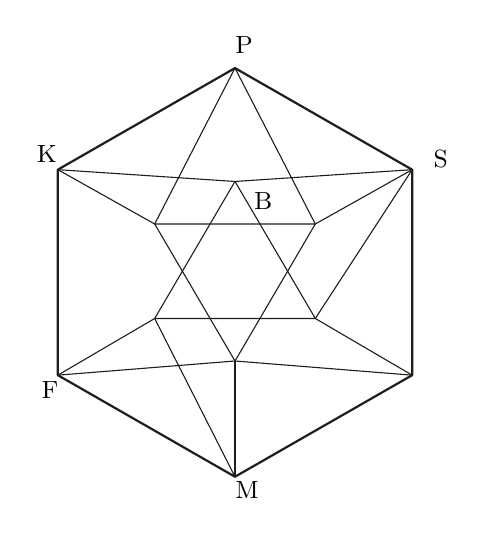
\begin{tikzpicture}[line cap=round,line join=round]
  \draw[msink,thick] (3.00,5.46) -- (5.25,4.17) -- (5.25,1.56) -- (3.00,0.27) -- (0.75,1.56) -- (0.75,4.17) -- cycle;
  \draw[msink] (3.00,4.02) -- (4.02,2.28) -- (1.98,2.28) -- cycle;
  \draw[msink] (3.00,1.74) -- (1.98,3.48) -- (4.02,3.48) -- cycle;
  \draw[msink] (3.00,5.46) -- (1.98,3.48);
  \draw[msink] (3.00,5.46) -- (4.02,3.48);
  \draw[msink] (5.25,4.17) -- (4.02,3.48);
  \draw[msink] (5.25,4.17) -- (4.02,2.28);
  \draw[msink] (5.25,1.56) -- (4.02,2.28);
  \draw[msink] (5.25,1.56) -- (3.00,1.74);
  \draw[msink] (3.00,0.27) -- (3.00,1.74);
  \draw[msink] (3.00,0.27) -- (1.98,2.28);
  \draw[msink] (0.75,1.56) -- (1.98,2.28);
  \draw[msink] (0.75,1.56) -- (3.00,1.74);
  \draw[msink] (0.75,4.17) -- (1.98,3.48);
  \draw[msink] (0.75,4.17) -- (3.00,4.02);
  \draw[msink] (5.25,4.17) -- (3.00,4.02);
  \node[anchor=base west] at (2.88,5.64) {\small P};
  \node[anchor=base west] at (0.36,4.26) {\small K};
  \node[anchor=base west] at (5.40,4.20) {\small S};
  \node[anchor=base west] at (0.42,1.26) {\small F};
  \node[anchor=base west] at (2.88,0.00) {\small M};
  \node[anchor=base west] at (3.12,3.66) {\small B};
\end{tikzpicture}
\mscaption{Redrawn after the marginal figure, which the scribe draws hatched and in perspective, its silhouette a hexagon.\footnote{The manuscript's figure is a small hatched drawing of the solid seen down a three-fold axis, so that its outline is a hexagon; the letters K, B, P, S, F and M are set round it, and D is the mid-point of the edge KB. The redrawing here keeps that projection and those letters.}}
\end{msfigure}

\dutchtext{Hoe groot is den inhoud van een Icosaëdrum,\footnote{\textit{Icosaëdrum} --- the hand's Latinised form; \textit{duijm} is the inch, twelve to the foot, and the only place on the paper where a measure other than the foot appears.} wiens eene zijde van de Grondvlakte als KB 30 duijm, en de geheele hoogte NM 48 duijme is? \textcolor{msred}{Antwoord 36 \vfrac{1}{9} cubic voete.}}
\engtext{How great is the content of an icosahedron, one side of whose base KB is 30 inches, and whose whole height NM is 48 inches? \textit{Answer: 36 \vfrac{1}{9} cubic feet.}}

\worktitle{Bewerking}{Working}
\begin{workblock}
  \wrow{
 
 
 
 }{$KP = 30$}{}
  \wrow{}{$KD^2 = 225$}{}\ruleunder
\end{workblock}

\reading{The paper ends on a Platonic solid, and on the only calculation that changes its units. The icosahedron is taken as twenty pyramids with their points at the centre: find one equilateral face by Pythagoras, take a sixth of the total height as the third of the half-height that the pyramid rule requires, multiply, multiply by twenty, and divide the cubic inches by 1728 to bring the answer to cubic feet. It is a fitting last question --- every technique the examination has taught is used at once, and the last thing it asks for, when all the geometry is done, is that a foot has twelve inches.}

\begin{msnotes}
  \item[3.] $\surd$675 is 25\textperiodcentered{}98, taken as 26; the face is then 15 $\times$ 26 = 390 square inches, against a true 389\textperiodcentered{}7. The proposition names the edge KB and the working uses KP, the two being the same edge of the same triangular face.
  \item[4.] A sixth of the whole height is a third of the half-height --- that is, a third of the height of each of the twenty pyramids running from a face to the centre. The examiner folds the pyramid rule's division by three into the fraction and says nothing about it. 390 $\times$ 8 = 3120; $\times$ 20 = 62,400 cubic inches; $\div$ 1728 = 36 \vfrac{1}{9} cubic feet, exact.
  \item[5.] \textcolor{msred}{The datum is impossible.} An icosahedron's height follows from its edge: it is twice the inradius, $\tfrac{a\sqrt3}{6}(3+\sqrt5)$, which for $a$ = 30 duim is 45\textperiodcentered{}35, not the 48 the question gives --- too large by 5\textperiodcentered{}85 per cent. The answer inherits the whole of that error: 36 \vfrac{1}{9} against a true $\tfrac{5}{12}(3+\sqrt5)a^{3}$ = 58,906 cubic inches, or 34\textperiodcentered{}09 cubic feet, so the model answer is 5\textperiodcentered{}93 per cent high. Every other answer in the section is exact for the rule used. The method is not at fault: fed the height such a solid actually has, the same working gives 390 $\times$ 45\textperiodcentered{}35 $\div$ 6 $\times$ 20 $\div$ 1728 = 34\textperiodcentered{}11 cubic feet, within seven parts in ten thousand of the true volume. The error is in the question, and since this manuscript is the examiner's own answer key it was the standard sent home for approval.
\end{msnotes}

\end{document}
